

%
% Exemplo de utiliza??o do modelo pgeeltex.
%
% por Miguel Moreto, 2011
%  
% Use por sua conta e risco.
%
% Defini??o da classe a ser utilizada:
\documentclass[oneside,normaltoc,espacoumemeio,PGTEXdissertacao]{pgeeltex}
% O significado das op??es ? apresentado no manual.

% Utilize tamb?m a op??o PGTEXdraft caso voc? queira gerar uma vers?o para a
% banca examinadora em tamanho A4 e para impress?o em somente u m dos lados da
% folha.
% Sempre mantenha seu Tex / Miktex atualizado.

\usepackage[brazil]{babel}
\usepackage[utf8]{inputenc}
\usepackage[pt,showend]{programma}
\usepackage{longtable}


% A linha abaixo chama o pacote hyperref, configurado para usar o programa 
% dvipdfm.exe na convers?o do .dvi para o .pdf. Se voc? utiliza outra forma de
% gerar o pdf, altere a linha abaixo com a op??o adequada. Veja o manual do 
% hyperref para saber as op??es dispon?veis e outras configura??es do pacote.

% Sugest?o: Gere o pdf utilizando o dvipdfm.exe que converte direto
% de dvi para pdf. Caso contr?rio, configure adequadamente o pacote hyperref.
\usepackage[dvips,linktocpage=true,pdfauthor={Alexander de Almeida Pinto},
pdftitle={Utilização das metaheurésticas GRASP e ILS aditivado com programção
linear para resolução do problema de construção de trilhos de aeronaves},
pdfsubject={PCTA},pdfcreator={LaTeX e Dvips}]{hyperref}
\usepackage[alf,abnt-emphasize=bf,abnt-etal-text=it,bibjustif,abnt-etal-cite=2,abnt-etal-list=0,abnt-url-package=hyperref,recuo=0.5cm]{abntcite}
 
% Se voc? quiser utilizar o estilo de cita??o num?rica, ex. [1], [2], comente a linha acima e use o c?digo que est? comentado nas 3 linhas abaixo:
  %\usepackage[num,bibjustif,recuo=1cm]{abntcite} 
  %\usepackage{colchetesrefs} % Coloca colchetes na lista de refer?ncias ao final do documento.
  %\citebrackets{[}{]}
% N?o esque?a do comando \bibliographystyle{abnt-num} antes the chamar o seu arquivo .bib. (\bibliography) ao final do documento para que a lista de refer?ncias tamb?m esteja no formato num?rico.

\usepackage{nomencl} % Pacote necess?rio para a lista de siglas. 
% O comando a seguir diz ao Latex para salvar as siglas em um arquivo separado:
\fazlistasiglas[Lista de Abreviaturas e Siglas] % Par?metro opcional ? o t?tulo da lista.

\usepackage[font={bf,small}]{caption}

\usepackage{graphicx}



%\renewcommand{\familydefault}{cmr}
% A seguinte linha evita algumas mensagens de warning por parte do hyperref.
% Comentar se o pacote hyperref n?o estiver sendo utilizado.
\pdfstringdefDisableCommands{\edef\uppercase{}}


% Os comandos a seguir ajustam o posicionamento dos floats (figures e tables).
\renewcommand{\floatpagefraction}{0.90}
\renewcommand{\topfraction}{0.95}
\renewcommand{\bottomfraction}{0.95}
\renewcommand{\textfraction}{0.05}
\setlength{\intextsep}{5pt}
\setlength{\textfloatsep}{5pt}
\setlength{\floatsep}{5pt}
%%%%%%%%% In?cio das defini??es iniciais %%%%%%%%%


\autor{Alexander de Almeida Pinto}
\titulo{Utilização das metaheurísticas GRASP e ILS aditivado com
programação linear para resolução do problema de construção de trilhos de
aeronaves}
\titlePGTEX{Titulo em ingles}
% T?tulo do documento \titlePGTEX{\LaTeX ~Thesis/Dissertation Example Using the \pgeeltex} % T?tulo do documento, em ingl?s.

% Nos 3 comandos abaixo o par?metro opcional entre [] pode ser preenchido para o caso de
% alguma dessas pessoas ser mulher. Se n?o especificado, vale o valor default.
%  Valores default: Orientador, Co-orientador e Coordenador.
\orientadorPGTEX[Orientador]{Dr.}{Lucídio dos Anjos Formiga Cabral}

%\coorientadorPGTEX[Co-orientadora]{Grau}{Nome do co-orientador}
\coordenadorPGTEX[Coordenadora]{Dra.}{Tatiana Aires Tavares} % Coordenador do PPGEEL

\areaconcentracaoPGTEX{Computação Distribuída} 
% ?rea de concentra??o 
\concentrationareaPGTEX{Distributed Computing} %
% ?rea de concentra??o em ingl?s

\palavraschavePGTEX{Transporte, PCTA, Metaheurística, Método Exato,GRASP, Rotas e Aeronaves}
% Palavras chave 
\keywordsPGTEX{Transportation, ARP,  metaheuristic, Exact Method, GRASP,Aircraft Routing}
% Palavras chave em ingl?s

% Instru??es para banca examinadora:
%   -> O primeiro membro da banca, definido pelo comando \bancaAPGTEX ? o presidente da banca
%      (provavelmente o orientador).
%   -> O segundo membro ser? automaticamente o Co-orientador se ele existir e for definido pelo
%      comando \coorientadorPGTEX
%   -> Os demais membros da banca s?o definidos pelos comandos \bancaBPGTEX, \bancaCPGTEX, \bancaDPGTEX e
%      \bancaEPGTEX.
%   -> Deixando os parametros dos comandos dos membros da banca vazios (exemplo \bancaAPGTEX{}), far?
%      com que as respectivas linhas de assinatura n?o apare?am.
%   -> Os comandos suportam um par?metro adicional, entre colchetes, onde ? colocado o grau de titula??o
%      do respectivo membro da banca. Se este par?metro adicional n?o for utilizado, ent?o o valor padr?o
%      "Doutor" ? atribuido.

\bancaAPGTEX[Dra.]{Tatiana Aires Tavares}
\bancaBPGTEX[Dr., UFPB]{Antonio Carlos Cavalcanti}
%\bancaCPGTEX{} % Como exemplo, o membro D da banca n?o vai aparecer por estar vazio.
%\bancaDPGTEX{}
%\bancaFPGTEX[Doutor, MIT]{Membro F da banca}
%\bancaGPGTEX[Doutor]{Membro G da banca}

\local{João Pessoa} 

\mesPGTEX[Ago]{Agosto} % Mes de publica??o
\anoPGTEX{2011} % Ano
\datadefesaPGTEX{04/08/2011} % Data da defesa.

% Dados para confec??o da capa de um trabalho de disciplina.
% Nescess?rios somente se a op??o de classe PGTEXtrabalho for utilizada.
\labPGTEX{LABSPOT}
\discipPGTEX{Disciplina 1}

%%%%%%%%% Fim das defini??es iniciais %%%%%%%%%

\begin{document} % In?cio do documento.

% Monta a capa (no novo modelo da BU, a capa ? feita separadamente, o texto inicia com a folha de rosto):
%\capaPGTEX

% Monta a folha de rosto:
\folhaderostoPGTEX
% Monta a folha de aprova??o:
\folhadeaprovacaoPGTEX

% DEDICAT?RIA
%
% Est?o dispon?veis dois tipos de dedicat?ria:
\begin{dedicatoriaPGTEX}
Dedico esse trabalho a minha família que me ajudou em todos os momentos
que precisei.
\end{dedicatoriaPGTEX}

% e / ou:



% EPIGRAFE (opcional).
% Parametro obrigatorio entre {} ? o autor da epigrafe.
\begin{epigrafePGTEX}{Bruce Calvert} 
Acreditar é mais fácil do que pensar. Daí existem muito mais crentes do que
pensadores.
\end{epigrafePGTEX}


% AGRADECIMENTOS
\begin{agradecimentosPGTEX}
Aqui entra os agradecimentos.
\end{agradecimentosPGTEX}

% RESUMO:
\begin{resumoPGTEX}
Os problemas operacionais cresceram muito em complexidade nos últimos
tempos, o que tem tornado necessário o desenvolvimento de técnicas que possam agilizar a tomada de decisão. Empresas que não utilizam sistemas 
computadorizados com essa finalidade tem perdido espaço entre seus concorrentes.
 
 A construção de trilhos de aeronaves é considerado um dos principais problemas da indústria aeronáutica e se 
 refere ao sequênciamento dos voos de uma companhia aérea de forma que o menor número de aeronaves seja necessário 
 para opera-las. Esse problema possui uma característica combinatória e a sua resolução fica mais difícil a medida 
 que a quantidade de voos envolvidos cresce. Entretanto pequenas modificações nos horários de partida desses voos, 
 ou o acréscimo de algum voo de resposicionamento entre dois aeroportos próximos podem gerar soluções de baixo custo.
 
 Apresentamos uma algoritmo híbrido baseado na metaheurística GRASP, com a utilização do ILS e de programação inteira 
 na busca local. Esse algoritmo é indicado para resolução de problemas de larga escala, pois nesse caso fica inviável 
 a aplicação de um algoritmo puramente exato que poderia levar anos para realizar a tarefa. Os resultados preliminares 
 tem mostrado agilidade na obtenção de boas soluções.
 \end{resumoPGTEX}

% ABSTRACT
\begin{abstractPGTEX}
Write here the English version of your Resumo... 
\end{abstractPGTEX}


\listadefiguras

\listadetabelas

\listadesiglas

%\listadesimbolos

\sumario
  
\chapter{Introdução}
  
 A aviação é o principal meio de transporte de pessoas e de mercadorias capaz
 de atravessar grandes distâncias além de ser fundamental para o crescimento
 da economia e do turismo mundial contribuindo assim para a melhora da
 qualidade de vida das pessoas proporcionando lazer e experiências com outras
 culturas. O uso da aviação comercial tem crescido significativamente nas
 últimas décadas e a previsão é que esse aumento seja cada vez maior, pelo
 menos no Brasil, que está fazendo um grande investimento para ampliar e
 melhorar a infraestrutura aeroportuária com a finalidade de atender a grande
 demanda que é esperada para a Copa do Mundo de 2014 e para as Olimpíadas de
 2016. Além disso a economia do país está crescendo e provocando um aumento da
 renda e da qualidade de vida incentivando as pessoas a viajar e explorar novas
 oportunidades.

%Pode se falar também do aumento da confiança no setor aereo que está sendo
% associado a uma forma segura de viajar.
  	
Esse ambiente favorável tem provocado o aumento do número de companhias
aéreas, fazendo com que ocorra uma maior competição e assim a necessidade de
otimizar a utilização dos recursos disponíveis, reduzindo os custos para
poder continuar a crescer e oferecer tarifas mais competitivas. Porém os
problemas presentes na indústria aeronáutica são complexos envolvendo
múltiplas decisões conflitantes que precisam ser otimizadas em conjunto.
Diversas técnicas são desenvolvidas e utilizadas para tentar melhorar o
planejamento e a operação das empresas aéreas. Muitas dessas técnicas estão
disponíveis na literatura científica, nos campos da pesquisa operacional e da
matemática e normalmente são modelados para funcionar em sistemas
computadorizados de alta capacidade com a finalidade de automatizar, ou pelo
menos auxiliar a tomada de decisões. Essas técnicas se tornam mais
necessárias a medida que a empresa aérea cresce e a tomada de decisão,
baseada nos julgamentos individuais e nas experiências, se tornam mais
difíceis \cite{ahmed2009}.
  	
  	
Os principais problemas relacionados dizem respeito ao planejamento, envolvendo
a criação de linhas de trabalho tanto para as aeronaves quanto para a
tripulação. O objetivo costuma ser a minimização dos custos operacionais ou a
maximização dos rendimentos. Custos operacionais consiste, por exemplo, nos
custos envolvidos com combustíveis, óleo, taxas de aterrissagem. Também pode
ser levado em consideração a perda de rendimentos com a utilização de aeronaves
com menos assentos do que a demanda de passageiros. Fatores como o bem
estar dos passageiros também pode ser levado em consideração, provocando por
exemplo a uma redução na quantidade de conexões e de escalas.
	
Para que seja possível ter uma visão geral do contexto é necessário descrever os
problemas que estão associados com a construção de trilhos de aeronaves. O
primeiro dos problemas que será tratado aqui é a modelagem de mercado que tem
como objetivo de fazer o levantamento da quantidade de passageiros que tem
interesse em viajar entre as localidades e em qual espaço de tempo,
adicionalmente pode-se criar demandas através da criação de novas rotas com o
auxilio de propagandas. Essa demanda normalmente apresenta uma grande variedade
dependendo da época do ano e o levantamento desses dados de forma errada pode
causar grandes prejuízos. É importante categorizar o tipo de passageiro para
poder fazer escolhas futuras que não levem em consideração apenas fatores
quantitativos.

Posterior a modelagem de mercado tem-se a necessidade de definir qual
equipamento (frota) irá operar cada trecho definido pela
demanda \cite{pimentel2005}, esse problema é conhecido como a atribuição de
frota (\textit{Fleet Assigment Problem}) . A definição de um equipamento errado
pode provocar a subutilização da aeronave o que provocaria prejuízos ou a
superutilização que provocaria insatisfação dos clientes. Ao final dessa etapa
irão ser formados conjuntos de voos que deverão ser operados por tipos de
aeronaves específicas. É a partir desses conjuntos que deverá ser feito a
construção dos trilhos das aeronaves.

Um trilho de aeronave é a sequência de voos que uma aeronave deve operar em um
determinado período, e o problema de construção desses trilhos 
(\textit{Aircraft Rotation Problem}) tem como objetivo principal a redução do
número de aeronaves necessários para operar todos os voos e como objetivo
secundário fazer o menor número de modificações possíveis no planejamento inicial desses
voos.

O passo seguinte utiliza das sequencias de voos do passo anterior para construir
o melhor conjunto de pairings\footnote{Pairing é o conjunto de voos
que pode ser operados por uma tripulação sem que seja violada qualquer
regra da legislação vigente e que ao final do último voo o tripulante
esteja de volta a sua cidade base.} de forma que cada voo seja coberto por
pelo menos um pairing. Gastos com alojamentos, alimentação, transporte em terra
e deadheads\footnote{Deadhead é o voo que o tripulante viaja sem trabalhar,
com a finalidade de transporte para outra localidade normalmente para sua
base ou para suprir uma nova demanda, o deadhead pode ser operado por
aviões de outras companhias, nesse caso o custo dessa viagem é maior.} devem
ser levados em consideração. A partir desse conjunto é feito a escala dos
tripulantes (\textit{Crew Scheduling Problem}) que atribui os pairings a
tripulação acrescentando as atividades de solo, tais como \textit{Call
Time}\footnote{Call time é o tempo que a tripulação tem para se apresentar a
companhia aérea antes de iniciar de fato seu turno de trabalho.},
\textit{Stand-by duties}\footnote{Stand-by duties
são turnos em que o tripulante fica a disposição da companhia aérea afim de
suprir possíveis eventualidades.} e os dias de descanso. O objetivo dessa ultima
etapa é fazer uma distribuição da forma mais justa possível, tentando balancear
a quantidade de trabalho (horas a serem voadas) entre os tripulantes e também
tentar cumprir as preferencias dos tripulantes sem violar nenhuma restrição da
legislação trabalhista em vigor.
   

Esse trabalho mostra uma forma eficiente de resolver o Problema de Construção
de Trilhos de Aeronaves (PCTA) 
%\abbrev{PCTA}{Problema de Construção de Trilhos de Aeronaves} 
que também é conhecido na literatura como Aircraft Rotation
Problem (ARP) 
%\abbrev{ARP}{Aircraft Rotation Problem}
. O PCTA é um dos
principais problemas presentes na industria da aviação e seu objetivo
é fazer o sequenciamento dos voos de cada frota da companhia de forma que seja
possível opera-las com o menor número de aeronaves possíveis\citep{abiliolivro}
bem como efetuar a menor modificação possível no planejamento inicial dos voos.
Cada sequência de voos recebe o nome de trilho de aeronave e o conjunto desses
trilhos é denominado de malha aérea. 

Para resolver o PCTA foram aplicados técnicas de metaheurísticas combinadas com
o método exato de programação linear através da criação de um modelo matemático
simplificado.

Essa estratégia foi escolhida pois com os computadores atuais não é possível
obter resultados com a aplicação apenas do modelo, que retorna o resultado
ótimo, pois o tempo necessário para resolver instâncias semanais do PCTA já é
considerado inviável. A utilização apenas de metaheurística foi uma alternativa
que foi levada em consideração no início, porém nos resultados práticos a
qualidade da solução se mostrou muito aquém da desejada. Dessa forma surgiu a
idéia de mesclar as duas técnicas, com a finalidade de obter a convergência do
modelo e a velocidade da metaheurística.

Na literatura tem-se observado um crescimento no número de trabalhos que se
utilizam de metaheurísticas híbridas como método de resolução de problemas
complexos de otimização combinatória apresentando soluções de alta qualidade
(ACRESCENTAR CITAções). Esse fato também aconteceu na resolução do PCTA.



%Para resolver o PCTA, devemos estar cientes de algumas restrições que envolvem
%tempo e espaço. Por exemplo, um voo não pode iniciar antes da chegada do voo
%que lhe antecede, nem de um local diferente da cidade de destino deste voo
%antecessor, esses exemplos são denominados respectivamente de restrições
%temporais e geográficas do problema. Há também a restrição de que um voo deve
%permanecer em solo, entre conexões, por um período de tempo que seja suficiente
%para fazer a troca de passageiros e abastecimento da aeronave e quando for o
%caso para a mudança da tripulação, esse tempo varia de acordo com o aeroporto e
%com o tipo de aeronave.

%Existe também a restrição de consistência que está presente em instâncias que
%possuem frequência. Nessas instâncias um voo pode aparecer em diversos dias.
%Dessa forma deve-se garantir que o horário de partida desse voo seja o mesmo em
%todos os dias que ele ocorrer, ou seja, caso alguma modificação seja feita no
%horário de partida sugerido desse voo, em um dos dias, então todos os outros
%dias da frequência também devem ser modificados.

%Outro aspecto importante diz respeito às restrições de manutenção. Sabe-se que
%um avião deve ter checagens periódicas. Oportunidades de realizar essas tarefas
%ocorrem apenas em algumas conexões potencialmente disponíveis. Como
%consequência, uma sequência de voos deve ser construída de forma que essas
%restrições não sejam violadas. A fim de incorporar essas restrições facilmente
%ao nosso framework, assumimos que as rotações são designadas a tipos não
%específicos de aeronave. Dessa forma, se uma aeronave tem necessidade de
%manutenção, um voo especial é criado com origem e destino na base de manutenção
%escolhida e com a sua duração exatamente igual ao tempo de manutenção 
%\cite{pontes2002}.

%	Vale ressaltar ainda que na resolução do PCTA deve-se levar em consideração as
%	particularidades especificas de cada companhia aérea como o número de aviões
%disponíveis na frota, o atraso máximo permitido nos voos, a quantidade máxima
%de voos que podem sofrer atraso, o número máximo de voos que podem ser
%cancelados, o número máximo de voos de reposicionamento que podem ser criados
%entre outros.
	
%De uma maneira geral, o principal objetivo do PCTA é a minimização do número de
%trilhos seguido da minimização do custo total dos trilhos gerados. Esse custo
%pode envolver diversos componentes, sendo o tempo médio diário de utilização
%das aeronaves um dos mais importantes \citep{abiliolivro}.
 
%###################################### 
%Aqui já nao descreve mais o problema.
%######################################
  
Nos dias de hoje, com o avanço da tecnologia e o aumento da competitividade
desenvolver soluções com melhor qualidade acaba se tornando um fator decisivo
para a permanência no mercado, tornando-se então necessário a obtenção de
soluções de forma mais rápida, mais barata e utilizando menos recursos. Por
causa da dificuldade que é inerente a essa classe de problemas a qualidade das
soluções obtidas manualmente são muito inferior em relação a melhor solução
possível. Outra característica que reforça a necessidade da obtenção de melhores soluções é o
aumento do tamanho e da complexidade das instâncias trabalhadas. A partir desse
cenário pode-se perceber a necessidade de utilização de técnicas de otimização.

  
%As metaheurísticas podem ser definidas como um conjunto de procedimentos de
%caráter geral, com capacidade de guiar o procedimento de busca, tornando-o
%capaz de escapar de ótimos locais. Elas têm como objetivo, encontrar uma
%solução tão próxima quanto possível da solução ótima do problema com baixo
%esforço computacional. Em geral, as metaheurísticas são bastante utilizadas na
%resolução de problemas de otimização. Esses problemas, também conhecidos como
%problemas NP-difíceis\abbrev{NP}{Non-Polinomial}, podem ser definidos como um
%conjunto de problemas para os quais ainda não existe um algoritmo que os
%resolvam de forma exata e em tempo polinomial \citep{maritan2009}. Para esses
%tipos de problemas o uso de métodos exatos é bastante restrito, uma vez que o
%esforço computacional para encontrar uma solução exata em instâncias reais é
%consideravelmente alto. Na prática, no entanto, é suficiente encontrar uma
%solução melhor que a utilizada no ambiente operacional.


%#############################################
%{\large >>>> Descrever em que tem se baseado a solução desse problema na literatura <<<<}
%Essa parte deveria ir para a revisão da literatura.
%#############################################

Em relação ao PCTA a literatura pesquisada \cite{ahmed2009} \cite{arguelo1007}
\cite{cordeau2001} \cite{mohamed2011} \cite{abiliolivro} mostra uma grande quantidade de
tentativas de resolver o problema utilizando modelagens matemáticas, que apesar
de garantir a solução ótima não se mostra viável para resolver grandes
instâncias. Alguns trabalhos mostram a similaridade desse problema com o
problema do caixeiro viajante assimétrico \cite{clarke97}. E outros resolvem
uma parte do problema utilizando metaheurísticas \cite{arguelo1007}. Além disso,
a pesquisa constatou que a literatura acerca do PCTA não disponibiliza as
instâncias que foram trabalhadas dificultando assim a comparação dos
resultados obtidos com esses trabalhos, logo um dos objetivos desse trabalho é
disponibilizar um conjunto de instâncias.

%#############################################
%{\large	>>>> Fazer uma breve descrição de programação linear, maiores detalhes serão dados na fundamentação teórica. <<<<	}
%#############################################

Atualmente existem diversas fontes na qual se podem obter instâncias para
problemas de otimização combinatória sendo uma das mais conhecidas a
OR-Library \footnote{ A OR-Library pode ser acessado em
http://people.brunel.ac.uk/~mastjjb/jeb/info.html} que foi descrito
inicialmente em J.E.Beasley \cite{orlibrary} permitindo o acesso a centenas de
conjuntos de instâncias a partir da Internet.
  
Apesar da existência dessas entidades apenas uma instância, a da Rio Sul, foi
encontrada em um relatório técnico da UFPB. Com a finalidade de ter outra
instância, foi feito em dezembro de 2010 o levantamento dos voos operados pela
compahia denominada TAM (http://www.tam.com.br). Esse levantamento foi feito
atarvés de uma pesquisa observativa através do comparativo da malha operada
pela companhia, que pode ser visto na Figura \ref{fig:malhatam}, e as
possibilidades de voos diretos do equipamento AirBus Industrie A310, que era a aeronáve com a maior frota da
empresa.
	
\begin{figure}[ht]
\caption{Rotas de voo da companhia aérea TAM. \mbox{Fonte:
(http://www.airlineroutemaps.com/)}}
\label{fig:malhatam}
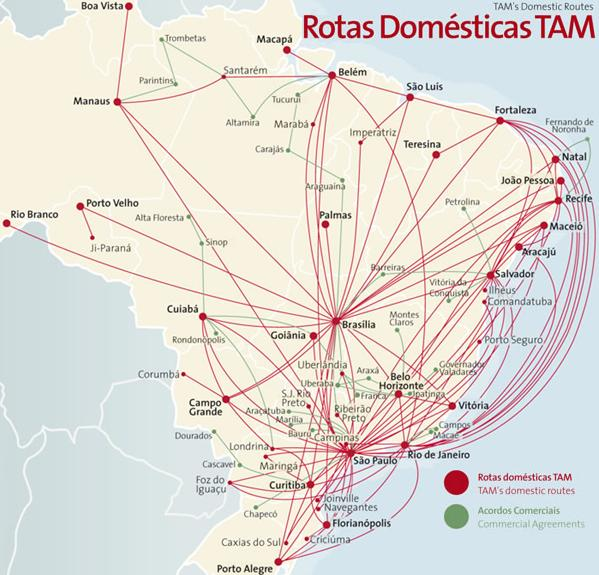
\includegraphics[scale=0.45]{./img/tam_brazilian_airlines}
\end{figure}
	
A malha da Rio Sul se refere a uma instância com voos de um dia de operação da
empresa contendo 107 voos, onde na prática era operado com 20 trilhos
que eram formados manualmente \cite{pontes2002}. A malha da TAM, que foi obtida
manualmente, é formada por 241 voos que possuem uma grande quantidade de
ligações entre os 31 aeroportos envolvidos, dessa forma o grau de complexidade
dessa instância se mostrou mais complexa. 

Essas instâncias foram estendidas para o período de uma semana para testar o
comportamento do algoritmo e do solver. Dessa forma a instância da Rio Sul
estendida apresentou 749 voo e a da Tam estendida ficou 1687 voos.
	
O maior interesse desse trabalho se encontra em instâncias locais
pois as instâncias de outras grandes empresas globais apresentam a
característica hub-and-spoke, que pode ser vista na Figura
\ref{fig:hubandspoke}. Uma malha é caracterizada como sendo do
tipo hub-and-spoke se ela apresentar uma grande concentração de voos em poucos
aeroportos e adicionalmente se um voo tem ligação com um hub ele não poderá ter
ligação com outros hubs a não ser que ele também seja um hub.
Instâncias com essa caractéristicas são mais fáceis de serem
resolvidas pois não apresentam a caractéristica explosiva no nível das malhas
de voos heterogêneas presente nas malhas de voos brasileiras.
	
\begin{figure}[ht]
\caption{Malha hub-and-spoke. \mbox{Fonte: (Própria)}}
\label{fig:hubandspoke}
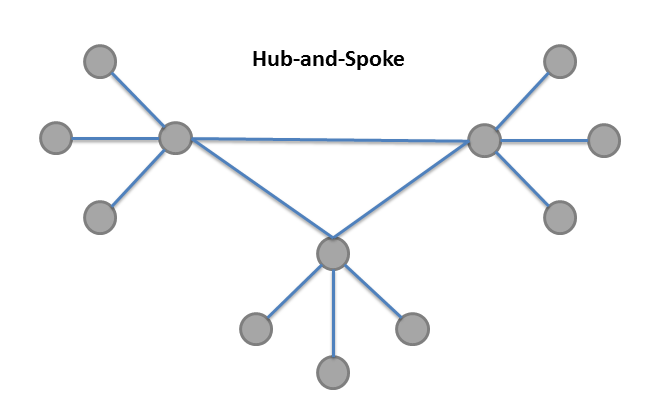
\includegraphics[scale=0.35]{./img/hubandspoke}
\end{figure}
 	 	
	
Novas instâncias reais não foram possíveis devido a falta de contato entre as
empresas e a acadêmia. Grande parte dessa falta de comunicação se deve ao receio
de revelar dados que podem vir a lhes prejudicar junto a concorrência.

Essas instâncias podem ser vistas nos anexos ao final desse trabalho.


\section {Objetivos do trabalho}

% Falar das consequências dos objetivos (em termo de economia e em relação a
% melhora do trafego aereo, no brasil, pois irá fazer com que as aeronáves
% fiquem mais tempo voando. O principal problema hoje é na falta de espaço no
% solo para pousar os avioes.

\subsection{Primário}
Tendo em vista os aspectos apresentados, o objetivo principal dessa proposta de
trabalho consiste no desenvolvimento de um método híbrido baseado nas
metaheurísticas GRASP e ILS e em programação linear inteira para a resolução do
problema construção de trilhos de aeronaves (PCTA) cobrindo todos os voos
planejados com o menor número de aeronaves bem como efetuando a menor mudança
possível no planejamento inicial desses voos. O método proposto tem a finalidade
de explorar a eficiência computacional, e irá ser combinada com etapas de
refinamentos composta por métodos exatos para acelerar a convergência e
adicionalmente fugir de mínimos locais.

\subsection{Secundário}

Esse trabalho também visa a disponibilização de um conjunto de instâncias que
irá permitir uma melhor comparação que poderá ser efetuada por trabalhos
futuros.

Adicionalmente disponibilizaremos uma interface que irá permitir ao usuário a
utilização de forma fácil do algoritmo com uma visualização do resultado através
de um gráfico de gantt.

\section {Organização da proposta }

O trabalho está estruturado da seguinte forma:

\begin{itemize}

\item Capítulo 1: Apresenta a motivação e as vantagens de resolver o PCTA
utilizando uma técnica híbrida com metaheurísticas e programação linear e
enfatiza a importância desse problema na indústria aeronáutica. Ao final os
objetivos do trabalho são descritos.

\item Capítulo 2: Apresenta a fundamentação sobre a otimização, metaheurísticas
e programação linear. Na seção referente à otimização além da descrição serão
discutidos heurísticas construtivas. A seção referente às metaheurísticas irá
iniciar com uma descrição seguida do detalhamento das metaheurísticas
utilizadas no trabalho, como o GRASP e o ILS. Ao final da fundamentação teórica
será feita uma revisão dos principais trabalhos relacionados ao presente
trabalho que estão presentes na literatura.

\item Capítulo 3: Mostra como foi obtida a malha da companhia de transporte aéreo TAM e qual a estratégia será utilizada para geração das novas instâncias.

\item Capítulo 4: Descreve o problema, explicando os conceitos que serão utilizados no trabalho.

\item Capítulo 5: Introduz o modelo matemático que foi desenvolvido.

\item Capítulo 6: Descreve o método proposto nesse trabalho, mostrando como foi feita a integração das metaheurísticas e da programação linear inteira e também descreve os parâmetros e as restrições que foram utilizadas.

\item Capítulo 7: Apresenta alguns resultados preliminares que já foram obtidos com o solver, dá diretrizes de como utilizar o método proposto e indica o que se espera ter para finalizar o trabalho.
%\item Capítulo 8: Dá uma conclusão, indicando o que tem que ser melhorado e o que se espera ter para a finalização do trabalho.

\item No final é apresentado a bibliográfia estudada, o cronograma de trabalho proposto durante os 24 meses de mestrado e os anexos que contém um maior detalhamento das instâncias e dos resultados obtidos.

\end{itemize}
\chapter{Fundamentação Teórica}

  Nesse capítulo será feita a fundamentação dos principais assuntos presentes nesse trabalho: a heurística construtiva, as metaheurísticas e a programação linear. Nas seções seguintes serão descritas os aspectos teóricos e os principais métodos relacionados a esse trabalho.

	\section{Heurísticas Construtivas}
		As técnicas de resolução heurísticas se utilizam de processos intuitivos com a finalidade de obter uma boa solução, a um custo computacional aceitável, ou seja não garante a otimalidade de um problema. O objetivo é obter em um tempo reduzido uma solução tão próxima quanto possível do ótimo global. 
		
		Uma heurística é dita construtiva quando a construção da solução se dá elemento por elemento. A forma de escolha dos elementos variam de acordo com a estratégia e a função de avaliação adotada, essa escolha deve levar em consideração o benefício da inserção de cada elemento para a solução final, escolhendo sempre o \emph{melhor} elemento em cada passo.
		
		O Algoritmo \ref{alg:heurconsgulosa} mostra o pseudocódigo para a construção de uma solução inicial para um problema de otimização que utiliza uma função gulosa \emph{g(.)}. Nesta figura, \emph{$t_{melhor}$} indica o membro do conjunto de elementos candidatos com o valor mais favorável da função de avaliação \emph{g}, isto é, aquele que possui o menor valor de \emph{g} no caso de o problema ser de minimização ou o maior valor de \emph{g} no caso de o problema ser de maximização.


\begin{pgrm}[h]
\begin{programma}
\ALGORITHM{$ConstruçãoGulosa(g(.), s$)}
\STATE s \GETS $\emptyset$;
\STATE Inicialize o conjunto $C$ de candidatos;
\WHILE{$C \neq \emptyset$}
\STATE $g(t_{melhor}) = melhor\{g(t) \mid t \in C\}$;
\STATE $s \GETS s \cup \{t_{melhor}\}$;
\STATE Atualize o conjunto $C$ de elementos candidatos;
\ENDWHILE
\STATE\RETURN $s$;
\ENDALGORITHM
\end{programma}
\caption{Heurística de construção gulosa de uma solução inicial}\label{alg:heurconsgulosa}

\end{pgrm}		
		

Uma outra forma de obter uma solução inicial é escolhendo os elementos candidatos aleatoriamente. Isto é, a cada passo, o elemento a ser inserido na solução é aleatoriamente selecionado dentre o conjunto de elementos candidatos ainda não selecionados. A grande vantagem desta metodologia reside na simplicidade de implementação. Segundo testes empíricos , a desvantagem é a baixa qualidade, em média, da solução final. Essa técnica é recomendada quando a característica do problema torna mais fácil o refinamento do que a construção de uma solução \citep{notasmarcone}. 

O Algoritmo \ref{alg:heurconsaleatoria} mostra o pseudocódigo para a construção de uma solução inicial aleatória para um problema de otimização.

\begin{pgrm}[h]
\begin{programma}
\ALGORITHM{$ConstruçãoAleatória(g(.), s$)}
\STATE s \GETS $\emptyset$;
\STATE Inicialize o conjunto $C$ de candidatos;
\WHILE{$C \neq \emptyset$}
\STATE Escolha aleatoriamente $t_{escolhido} \in C$;
\STATE $s \GETS s \cup \{t_{escolhido}\}$;
\STATE Atualize o conjunto $C$ de elementos candidatos;
\ENDWHILE
\STATE\RETURN $s$;
\ENDALGORITHM
\end{programma}
\caption{Heurística de construção aleatória de uma solução inicial}\label{alg:heurconsaleatoria}
\end{pgrm}

Para melhores resultados essa etapa deve ser seguida de um refinamento, pois a solução, quando gerada aleatoriamente, não costuma ser de boa qualidade.

\section{Metaheurística}

A utilização de métodos exatos para a resolução de problemas reais envolvendo otimização combinatória é restrito. Isso acontece pois com o aumento das instâncias envolvidas, o número de soluções possíveis cresce exponencialmente, fazendo com que as operações necessárias para a sua resolução não possa feita em tempo viável com os computadores atuais.  

Para contornar essa limitação e obter soluções para esses tipos de problemas, os pesquisadores desenvolveram técnicas que são capazes de guiar o procedimento de busca e assim encontrar boas soluções \cite{maritan2009}. Esses algoritmos, denominados heurísticas, encontram essas soluções utilizando pouco recursos computacionais, porém não garantem a solução ótima do problema \cite{dias2006}. Na prática, geralmente, uma boa solução é suficiente, já que a tomada de decisão tem que acontecer em um curto espaço de tempo.

As heurísticas só se aplicam a uma classe restrita de problemas. Para contornar essa restrição, foram desenvolvidas técnicas mais generalistas que foram denominadas de metaheurísticas. As metaheurísticas podem ser definidas como sendo um método heurístico para resolver de forma genérica problemas de otimização com a capacidade de escapar de ótimos locais. A idéia utilizada, normalmente, é obtida de algum evento natural como sistemas biológicos, da física, da inteligência artificial entre outros.

As metaheurísticas podem explorar o espaço de soluções basicamente de duas formas: as metaheurísticas de busca local e as metaheurísticas de busca populacional. Nas metaheurísticas de busca local, o procedimento de busca utiliza uma solução como ponto de partida em cada iteração. As metaheurísticas GRASP, Arrefecimento simulado (Simulated Annealing), Busca Tabu e ILS podem ser citadas como exemplos de metaheurísticas ponto-a-ponto. Nas metaheurísticas de busca populacionais, soluções de boa qualidade são combinadas com o intuito de produzir soluções melhores. Podemos citar como exemplo de métodos populacionais, os Algoritmos Genéticos, Colônia de Formigas (Ant Colony System), Núvem de Particulas (Particle Swarm Optimization) e etc \cite{maritan2009}.

Nesse trabalho foram utilizados as metaheurísticas de busca local GRASP e ILS de forma híbrida. As próximas seções descrevem essas metaheurísticas.

\subsection{GRASP}

Essa seção descreve a metaheurística GRASP (Greedy Randomized Adaptive Search Procedure - Procedimento de busca adaptativa gulosa e randômica), que foi proposto por Feo e Rezende \cite{resende1995}, e cujos conceitos serão utilizados na metodologia proposta para resolução do PCTA.
A metaheurística GRASP é um método iterativo do tipo \textit{multi-start} formado por duas fases: uma fase de construção de uma solução e outra de busca local. A fase de construção objetiva gerar uma solução viável para o problema proposto. E a fase de busca local na qual um ótimo local na vizinhança da solução construída é pesquisado. A melhor solução encontrada, ao longo de todas as iterações GRASP realizadas, é retornada.

O pseudo-código descrito no Algoritmo \ref{alg:grasp} ilustra um procedimento GRASP para um problema de minimização. Na linha 1 o custo da função objetivo da melhor solução encontrada é inicializada com $\infty$. A linha 2 repete o procedimento de construção e refinamento $GRASPMax$ vezes, por causa dessa etapa que o GRASP é considerado \textit{multi-start}.

Na linha 3 e 4 são feitas respectivamente a construção e a busca local que são representadas nos Algoritmos \ref{alg:graspcons} e \ref{alg:grasplocal} e serão detalhadas mais adiante.

Nas linhas 5 à 8, se a solução obtida na busca local for melhor que a melhor solução obtida até o momento ($f(s) < f{*}$) então são atualizadas respectivamente a solução e o custo relativo a função objetivo dessa solução. 
A linha 9 encerra as iterações do GRASP e a linha 10 retorna a melhor solução obtida.

\begin{pgrm}[h]
\begin{programma}
\ALGORITHM{GRASP($f(.), g(.), N(.), GRASPMax, s$)}
\STATE f{*} \GETS $\infty$;
\FOR{$1, 2, ..., GRASPMax$}
\STATE Construção($g(.), \alpha, s$);
\STATE BuscaLocal($f(.),N(.),s$);
\IF{$f(s) < f{*}$}
\STATE $s{*} \GETS s$;
\STATE $f{*} \GETS f(s)$;
\ENDIF
\ENDFOR
\STATE\RETURN $s{*}$;
\ENDALGORITHM
\end{programma}
\caption{Procedimento GRASP.}\label{alg:grasp}
\end{pgrm}

Na fase de construção uma solução é iterativamente construída, elemento por elemento. A parte gulosa da função visa gerar uma solução factível de melhor custo. O componente aleatório é incluído para explorar
regiões diversas do espaço de soluções e é uma das chaves da efetividade do GRASP.

A fase de construção do GRASP é baseada na construção de uma lista restrita de candidatos (LCR). Essa lista contem os melhores candidatos que podem ser adicionados a solução em um dado momento, a quantidade de elementos dessa lista é regulada pelo $\alpha$ que é um dos parâmetros do GRASP. O $\alpha$ é definido como sendo o nível de aleatoriedade da solução.

\begin{pgrm}[h]
\begin{programma}
\ALGORITHM{$Construção(g(.), \alpha,s$)}
\STATE s \GETS $\emptyset$;
\STATE Inicialize o conjunto $C$ de candidatos;
\WHILE{$C \neq \emptyset$}
\STATE $g(t_{min}) \GETS min\{g(t) \mid t \in C\}$;
\STATE $g(t_{max}) \GETS max\{g(t) \mid t \in C\}$;
\STATE $LCR \GETS \{t \in C \mid g(t) \leq g(t_{min}) + \alpha(g(t_{max}) - g(t_{min}))\}$;
\STATE Selecione aleatoriamente um elemento $t \in LCR$;
\STATE $s \GETS s \cup \{t\}$;
\STATE Atualize conjunto de candidatos;
\ENDWHILE
\STATE\RETURN $s$;
\ENDALGORITHM
\end{programma}
\caption{Procedimento de construção do GRASP.}\label{alg:graspcons}
\end{pgrm}

Em cada iteração dessa são selecionados todos os elementos que podem ser inseridos na solução e então é formada uma lista de candidatos que é ordenada segundo algum critério de ordenação pré-determinado, no caso de um problema de minimização a lista normalmente é ordenada de acordo com o acréscimo na função objetivo que esse elemento acarretaria se fosse escolhido de forma gulosa. A heurística
é dita adaptativa porque os benefícios associados com a escolha de cada elemento são atualizados em cada iteração da fase de construção para refletir as mudanças oriundas da seleção do elemento anterior. A componente probabilística do procedimento reside no fato
de que cada elemento é selecionado de forma aleatória a partir de um subconjunto restrito formado pelos melhores elementos que compõem a lista de candidatos. Este subconjunto recebe o nome de lista de candidatos restrita (LCR). Esta técnica de escolha permite que
diferentes soluções sejam geradas em cada iteração GRASP \cite{notasmarcone}. O valor do grau de aleatoriedade $\alpha$ se encontra entre [0,1].

Um valor de $\alpha = 0$ faz com que o algoritmo gere soluções puramente gulosas enquanto a escolha de um $\alpha = 1$ faz com que o algoritmo gere soluções puramente aleatórias.
 
A construção do GRASP difere do Algoritmo \ref{alg:heurconsgulosa} por causa das linhas 4 à 7. A linha 4 obtém o valor mínimo que será acrescentado a solução final, dentre os candidatos possíveis e a linha 5 obtém o valor máximo. A linha 6 forma a LCR com os elementos que tiverem o valor entre $g(t_{min}) + \alpha(g(t_{max}) - g(t_{min}))$. Por fim a linha 7 seleciona aleatoriamente um elemento da LCR.

Com isso a quantidade de soluções possíveis é ampliada porém somente soluções promissoras são geradas.

As soluções geradas pela fase de construção do GRASP normalmente não são localmente ótimas com relação à definição de vizinhança adotada. Surge então a necessidade de complementar o método com a adição de uma busca local, que tem como objetivo melhorar a solução construída na fase de construção. O Algoritmo \ref{alg:grasplocal} descreve um procedimento básico de busca local relativo a uma vizinhança $N(.)$ de $s$ para um problema de minimização. A qualidade da construção gerada causa um impacto direto na busca local, uma vez que essa solução inicial podem constituir pontos de partidas promissores para a busca local, permitindo assim agiliza-los.

\begin{pgrm}[h]
\begin{programma}
\ALGORITHM{BuscaLocal($f(.), N(.), s$)}
\STATE $V \GETS \{s{'} \in N(s) \mid f(s{'}) < f(s)\}$;
\WHILE{$\mid V \mid > 0$}
\STATE Selecione $s{'}$ de $V$;
\STATE $s \GETS s{'}$;
\STATE $V \GETS \{s{'} \in N(s) \mid f(s{'}) < f(s)\}$;
\ENDWHILE
\STATE\RETURN $s$;
\ENDALGORITHM
\end{programma}
\caption{Procedimento de busca local do GRASP.}\label{alg:grasplocal}
\end{pgrm}

O algoritmo de busca local define no passo 1 e 5 o conjunto de vizinhos da solução que melhoram o valor da função objetivo. Do passo 2 à 6 a solução corrente é atualizada enquanto houver uma solução melhor na vizinhança. 

O GRASP apresenta basicamente o parâmetro $\alpha$ que pode ser ajustado. Valores de $\alpha$ que levem a uma LCR com tamanho bastante limitado (isto é, valor próximo da escolha gulosa) implicam soluções próximas as da solução gulosa, obtidas com um baixo esforço computacional. Porém, provocam uma baixa variedade de soluções construídas, que normalmente não é interessante para a busca local já que as soluções geradas são muito próximas. Por outro lado a escolha de valores de $\alpha$ muito elevados implicam na geração de uma grande diversidade de soluções mas, por outro lado, muitas das soluções construídas são de baixa qualidade.

Procedimentos GRASP mais sofisticados levam em consideração a mudança do valor de $\alpha$ ao longo das iterações. De acordo com os resultados obtidos em iterações anteriores. Estudos feitos em \cite{prais2000} indicam que essa adaptação do valor de $\alpha$ produz soluções melhores do que aquelas obtidas considerando-o fixo.

\subsection{ILS}

Essa seção descreve a metaheurística ILS (Iterated Local Search - Busca Local Iterativa) que se baseia na idéia de que um procedimento de busca local consegue melhores resultados quando a medida que a solução base é variada. Esses locais diferentes são obtidos a partir de pertubações em cima da solução ótima local corrente.

O Algoritmo \ref{alg:ils} ilustra o pseudo-código do ILS. Nele pode-se perceber a necessidade da definição de quatro procedimentos: (a) $GeraSoluçãoInicial()$ que obtém o ponto de partida $s_{0}$ para o problema; $BuscaLocal(s)$, que retorna o mínimo local da solução $s$, tendo como base as estruturas de vizinhança definidas; (c) $Pertubação(histórico, s)$, que altera a solução $s$ para outra solução, e se utiliza do histórico para evitar repetir soluções bem como para inferir o grau de pertubação necessário para escapar do mínimo local. E o (d) $CritérioDeAceitação(s, s{''}, histórico)$, que decide em qual solução a próxima pertubação será aplicada.

\begin{pgrm}[h]
\begin{programma}
\ALGORITHM{ILS}
\STATE $s_{0}$ \GETS GeraSoluçãoInicial;
\STATE $s$ \GETS BuscaLocal($s_{0}$);
\WHILE{os critérios de parada não estiverem satisfeito}
\STATE $s{'}$ \GETS Pertubação($histórico, s$);
\STATE $s{''}$ \GETS BuscaLocal($s{'}$);
\STATE $s$ \GETS CritérioAceitação($s, s{''}, histórico$);
\ENDWHILE
\STATE\RETURN $s$;
\ENDALGORITHM
\end{programma}
\caption{Procedimento Iterated Local Search.}\label{alg:ils}
\end{pgrm}

O ILS é dependente da escolha do método de busca local, das pertubações e do critério de aceitação. Normalmente um método de descida é utilizado, mas também é possível aplicar algoritmos mais sofisticados como Busca Tabu ou outras metaheurísticas.

A intensidade da perturbação deve ser forte o suficiente para permitir escapar do ótimo
local corrente e permitir explorar diferentes regiões. Ao mesmo tempo, ela precisa ser fraca
o suficiente para guardar características do ótimo local corrente \cite{notasmarcone}.

Um aspecto importante do critério de aceitação e da pertubação é que eles induzem aos procedimentos de intensificação e diversificação. A intensificação consiste em procurar melhores soluções nas área de busca corrente, isso acontece reduzindo a força da pertubação que faz com que as novas soluções de partida se encontrem nas proximidades da anterior. A diversificação acontece com a aplicação de grandes pertubações.

\begin{figure}[ht]
	\centering
	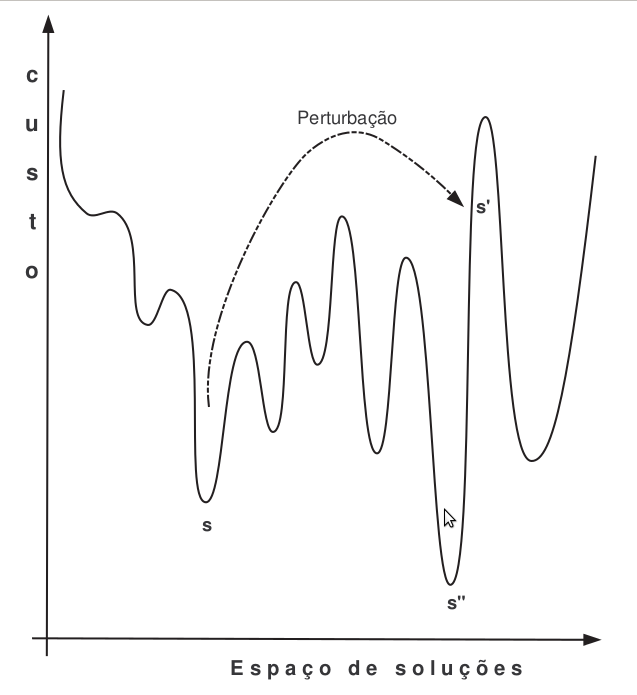
\includegraphics[scale=0.3]{./img/ilsfuncionamento.png}
	\caption{Representação esquemática do funcionamento do ILS}
	\label{img:ilsfuncionamento}
\end{figure}

A Figura \ref{img:ilsfuncionamento} demonstra o funcionamento do método ILS em um problema de minimização. Dado um ótimo local $s$, é realizada uma pertubação que lhe direciona para $s{'}$. Depois da aplicação da busca local, o novo mínimo $s{''}$, melhor que a anterior, é encontrada. Ou seja $f(s{''}) < f(s)$.

Uma exemplo de pertubação seria a aplicação sucessiva de estruturas de vizinhança a solução corrente.

\section{Programação Linear}

A programação linear é provavelmente a mais conhecida e utilizada técnica de otimização em todo o mundo. É geralmente utilizada para tomada de decisões gerenciais sobre a alocação de recursos para produção. Os custos dos recursos e as receitas geradas pelos produtos são usados para determinar a melhor solução. Qualquer problema que possa ser formulado com variáveis de decisão reais, tendo uma função-objetivo linear, e funções de restrição lineares, em princípio pode ser solucionado através da programação linear. Tais programas originariamente utilizavam o método \textit{Simplex}, porém, mais recentemente, métodos de "\textit{pontos interiores}" se mostraram mais eficientes.

Embora a programação linear seja muito eficiente para a resolução de problemas lineares, sua aplicação a problemas que apresentem objetivos ou restrições não-lineares tem levado a problemas e falhas de modelagem. Em alguns casos, funções não-lineares podem ser aproximadas por algumas funções lineares conjugadas, e a programação linear ainda pode ser utilizada. Contudo, isso leva a uma representação ineficiente do problema, podendo causar matrizes de decisão explosivamente grandes que demandam um tempo excessivo para resolução. Esta é uma dificuldade comum em problemas que envolvem, por exemplo, "\textit{scheduling}" e "\textit{sequenciamento}" de processos.

De forma equivalente, outros tipos de variáveis não podem ser tratadas diretamente com o uso de programação linear. Programação inteira usa programação linear para resolver problemas sobre variáveis inteiras, mas ainda com funções objetivo e restrições puramente lineares. As variáveis inteiras são representadas como variáveis reais no algoritmo de resolução do problema. Então um processo repetitivo é usado para "delimitar" o valor destas variáveis em valores inteiros, através da adição de restrições e reprocessamento da solução. Esse método, conhecido como \textit{"branch \& bound"}, finaliza quando todas as variáveis assumem valores inteiros. Quando o número de variáveis inteiras é pequeno, a programação inteira soluciona o problema rapidamente. Infelizmente esse procedimento pode consumir muito tempo com um número grande de variáveis inteiras, podendo, em alguns casos, necessitar de milhões de iterações para serem resolvidos.
 	
 	Essa técnica foi muito utilizada na segunda guerra mundial para otimizar as perdas inimigas e reduzir o custo das operações e também é utilizado no planejamento de algumas empresas.

\section{Revisão da literatura}
	
		O Trabalho de Argüello e Bard \citep{arguelo1007} (1997) resolve a parte de reconstrução de uma solução do PCTA que tenha sido corrompida por causa de atrasos e impedimentos de voos que ocorrem durante a execução de uma malha. Ele resolve esse problema utilizando a metaheurística GRASP, gerando vizinhos da solução atual de forma sucessiva até obter uma que seja considerada suficientemente boa.
		
		Mercier e Soumis \cite{mercier2007} (2007) resolveram o PCTA em conjunto com o problema de escala de tripulantes pois Cordeau et al. \cite{cordeau2001}, Klabjan et al. \cite{klabjan2002} e Cohn e Barnhart \cite{mainville2003} mostraram que a resolução desses problema de forma integrada pode gerar soluções que são significantemente melhor que as geradas de forma sequencial. O Modelo matemático proposto em CITAR AQUI foi adaptado para auxiliar na geração da nossa solução. 
		
		Em \cite{mohamed2011} Mohamed et al. resolveu de forma integrada o problema de atribuição de frota e o problema de construção de trilhos de aeronaves, para uma pequena empresa de aviação a TunisAir. Além disso as restrições de manutenção não foram levadas em consideração pelo fato dela poder ser feita em todos os aeroportos em que as aeronaves passam a noite.
		
%GRASPs have been used to find high quality solutions to a variety of logistics and combi- natorial optimization problems including maintenance base %planning (Feo and Bard, 1989), machine scheduling (Feo et al., 1991), and number partitioning (Argu ̈ello et al., 1996) to name a few.


\chapter{Revisão da literatura}
  
\cite{arguelo1997} apresenta um algoritmo, baseado no GRASP, para reconstruir
trilhos de aeronaves que tenham sofrido modificações durante o decorrer do dia.

Para isso ele usa uma função de avaliação gulosa e um método de seleção
aleatório que de forma iterativa tenta construir uma solução viável, a
solução inicial é utilizada como entrada e então é viabilizada através desses
movimentos. Note que se a solução inicial ainda for válida, a fase de construção
se torna desnecessária. 

Em cada iteração os movimentos possíveis são gerados e
avaliados. Os mais promissores são armazenados na lista restrita de candidatos
(LRC) na qual uma é selecionada aleatoriamente. A LCR pode ser restringida por
quantidade ou por qualidade. Por exemplo, os melhores $X$ movimentos ou todos os
movimentos com $Y$\% do melhor movimento podem ser armazenados na LRC.
Esse processo é repetido até que uma solução válida seja obtida. Isto
representa uma iteração. A vantagem de usar a solução inicial é que ela é
próxima a malha aérea planejada inicialmente pela companhia. 

A fase de busca local usa a solução da fase de construção para encontrar um
mínimo local. Essa fase usa procedimentos de trocas determinísticas para
atingir o mínimo local. 

A vizinhança definida inclui a criação de um novo  conjunto de trilhos em que os
voos que forem alocados a eles serão cancelados. Três são as operações usadas
para gerar novos vizinhos: \textit{flight route augmentation}, \textit{partial
route exchange}, e \textit{simple circuit cancellation}. Os dois primeiros são
aplicados em um par de trilhos e o terceiro é aplicado em um único trilho. 

O \textit{flight route augmentation} opera removendo um voo ou uma sequência de
voos de um dos trilhos e adicionando esses voos no outro. O trilho de destino é
aumentado dos voos removidos do trilho de origem. O trilho de destino pode ser
aumentado de três formas distintas. Primeiro, um circuito pode ser colocado no
seu início. Um circuito é uma sequência de voos que inicia e termina no mesmo
aeroporto. Uma segunda forma é inserir o circuito em algum lugar entre o
primeiro e o último voo do trilho de destino. A terceira forma permite alterar
o aeroporto de destino, ou seja, insere uma sequência de voos no trilho de destino. 

O \textit{partial route exchange} opera simplesmente trocando um par de
sequências de voos entre dois trilhos e o \textit{simple circuit cancelation}
remove um circuito de um trilho e cria um trilho de cancelamento. 

Os testes realizados no artigo foram feitos em uma instância cedida pela
Continental Airlines, referente a frota 757, com 42 voos operados por 16
aeronaves em uma rede de 13 aeroportos espalhados por 3 continentes. A malha
não foi disponibilizada no artigo.

		
\cite{mercier2007} desenvolveram um modelo matemático que permite resolver de
forma integrada a construção de trilhos de aeronaves e a escala de tripulantes
permitindo mudanças nos horários dos voos. A ligação entre as restrições desses
dois problemas garante que o mesmo planejamento seja feito para os trilhos das
aeronaves e para a escala dos tripulantes, permitindo assim a redução de custos
pela antecipação de problemas das etapas futuras. Por outro lado essa abordagem
aumenta a complexidade na resolução desses problemas. Com a agregação desses
dois problemas a resolução se tornou pesada e viável apenas para instâncias
diárias. Os testes do algoritmo foram baseados em instâncias contendo no máximo
500 voos que foram fornecidas por duas grandes companhias aereas, os dados
dessas instâncias não se encontram disponíveis no artigo.

\cite{cordeau2001}, \cite{klabjan2002} e \cite{mainville2003} mostraram em seus
trabalhos que a resolução desses problemas de forma integrada podem gerar
soluções que são significativamente melhores que as obtidas pela resolução
sequencial.

  		
Pontes R., et al \cite{pontes2002} utilizaram a fase de construção do GRASP
para resolver o PCTA, também propuseram um modelo matemático que foi
adaptado para auxiliar na geração da nossa solução. Além disso, uma instância
da Rio-Sul foi disponibilizada para a realização de testes. Com o solver eles
conseguiram obter a solução ótima dessa instância mas o autor informou que
essa resolução demorou dias para finalizar. Com a utilização da heurística
eles conseguiram apenas se aproximar dessa solução porém com um tempo de 384
segundos. 
		
Em \cite{mohamed2011} Mohamed et al. resolveu de forma integrada o problema
de atribuição de frota e o problema de construção de trilhos de aeronaves,
para uma pequena empresa de aviação a TunisAir. Além disso as restrições de
manutenção não foram levadas em consideração pelo fato dela poder ser feita
em todos os aeroportos em que as aeronaves passam a noite.
		
%GRASPs have been used to find high quality solutions to a variety of logistics and combi- natorial optimization problems including maintenance base %planning (Feo and Bard, 1989), machine scheduling (Feo et al., 1991), and number partitioning (Argu ̈ello et al., 1996) to name a few.
%ão
 
\chapter{Descrição do problema}\label{cap:descprob}

%%%Aqui é a descrição do problema - Opcionalmente pode virar um capitulo.
  Os voos são organizados de forma que cada aeronave seja responsável por uma sequência válida, que é chamada de trilho.  O conjunto desses trilhos é a solução do problema e é denominada de malha. Essa malha deve conter o menor número possível de trilhos que atenda todos os voos planejados com o mínimo de modificações em relação ao planejamento inicial.
  
  As restrições que envolvem o PCTA induzem a formação de uma rede de possíveis conexões. Nessa rede os nós representam os voos e os arcos representam as conexões possíveis entre esses voos. Dessa forma o problema pode ser formulado como um problema de minimização de fluxos em uma rede.
  
  Dado a possibilidade de mudanças no tempo de partida sugerido dos voos e também a permissão para criar voos de reposicionamento, uma grande quantidade de soluções podem ser geradas. A ligação dos voos pode ocorrer de 6 formas distintas aqui denominado tipos de arcos. Os  arcos do tipo 1 permitem a ligação de voos sem a utilização de atrasos e/ou reposicionamento. Os arcos do tipo 2 utilizam atrasos mas não o reposicionamento. Os arcos do tipo 3 permitem o sequenciamento com a utilização de um voo de reposicionamento mas sem inserir atraso em nenhum dos voos envolvidos. Os arcos do tipo 4 utilizam-se de atrasos e de um voo de reposicionamento para fazer a ligação entre dois voos. Os arcos do tipo 5 e 6 são usados no modelo, que é baseado no fluxo em grafo, para representar respectivamente o nó origem(source) e o destino(sink). Abaixo um maior detalhamento desses arcos:

  
  \begin{itemize}
\item Conexão natural (Arco do tipo 1) - Os arcos desse tipo conectam dois voos respeitando o tempo de partida sugerido e
a restrição geográfica. Eles são associados com as ligações que não requerem mudanças no tempo de partida e nem
       precisam de voos de reposicionamento. O arco do tipo 1 não apresenta custo para ser adicionado a solução.

\begin{figure}[ht]
	\centering
	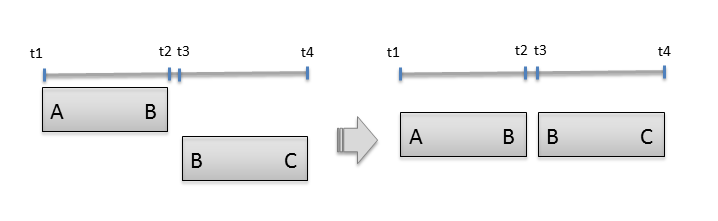
\includegraphics[scale=0.35]{./img/arc1}
	\caption{Representação esquemática do arco do tipo 1}
	\label{fig:arc1}
\end{figure}

\item Mudança no tempo (Arco do tipo 2) - Apesar de ter os voos incidentes no mesmo aeroporto, os arcos desse tipo não
permitem a ligação de forma direta pois o tempo de solo disponível não é suficiente para permitir a ligação. No
      entanto, a escolha desse tipo de arco implica em uma mudança no tempo de partida sugerido para quaisquer um dos
      voos envolvidos. O custo de um arco desse tipo é igual a soma dos valores absolutos dos atrasos (em minutos) dos
      horários de partida envolvidos.
      
\begin{figure}[ht]
	\centering
	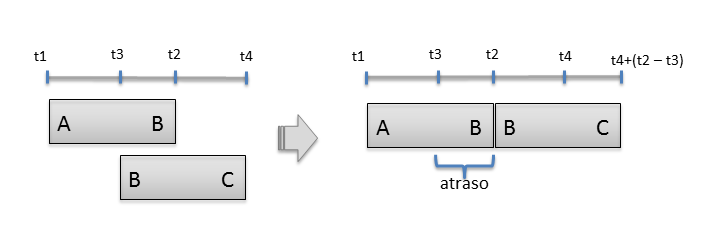
\includegraphics[scale=0.35]{./img/arc2}
	\caption{Representação esquemática do arco do tipo 2}
	\label{fig:arc2}
\end{figure}

\item Voos de reposicionamento (Arco do tipo 3) - Esses arcos representam conexões entre dois voos em que a origem
parte de um aeroporto diferente do local de partida do voo de destino, no entanto, existe tempo suficiente para um voo
de reposicionamento, entre os dois locais, sem violar as restrições de tempo de solo. Os custos de um arco do tipo 3 é
  igual a duração do voo de reposicionamento, incluindo o seu tempo de solo.

\begin{figure}[ht]
	\centering
	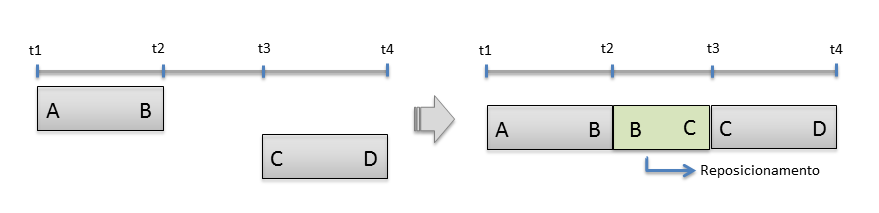
\includegraphics[scale=0.35]{./img/arc3}
	\caption{Representação esquemática do arco do tipo 3}
	\label{fig:arc3}
\end{figure}

\item Voos de reposicionamento mais mudança de tempo (Arco do tipo 4) - Esses arcos representam conexões que
precisam de um voo de reposicionamento mais mudança no tempo de partida sugerido. O arco do tipo 4 tem custo
igual tempo do voo de reposicionamento, incluindo o tempo de solo, mais a soma dos atrasos dos horários de partida
envolvidos em valor absoluto.

\begin{figure}[ht]
	\centering
	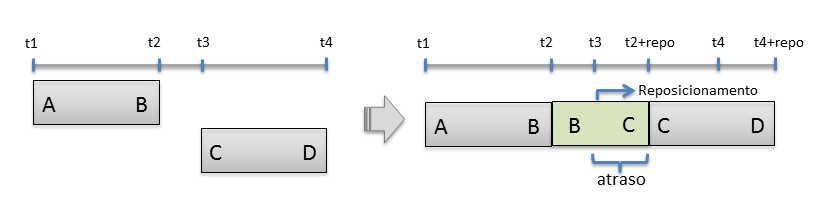
\includegraphics[scale=0.35]{./img/arc4}
	\caption{Representação esquemática do arco do tipo 4}
	\label{fig:arc4}
\end{figure}

\item Arcos do nó fonte ou \textit{source} (Arco do tipo 5) - Esses, arcos são criados para identificar o inicio de um trilho e é com
 ele também que se sabe a quantidade de trilhos necessários para resolver o problema. Cada arco do tipo 5 tem o custo
  igual a 1000.

\item Arcos do nó final ou \textit{sink} (Arco do tipo 6) - Esses arcos tem como destino o nó fictício que é usado para finalizar um
  trilho no modelo. Os arcos do tipo 6 não tem custo.

\end{itemize}

Abaixo na Figura \ref{fig:arpexample} temos dois exemplos de montagem de trilhos feitas a partir de um conjunto fictícios de voos. Cada caixinha laranja e azul representa um voo, onde a parte laranja representa o tempo de solo que cada voo deve obedecer e a azul seria o tempo de voo da cidade de origem para a cidade de destino. As letras A, B, C, D, E representam as cidades e a linha pontilhada indica o tempo de inicio e de termino de cada voo.

\begin{figure}[ht]
	\centering
	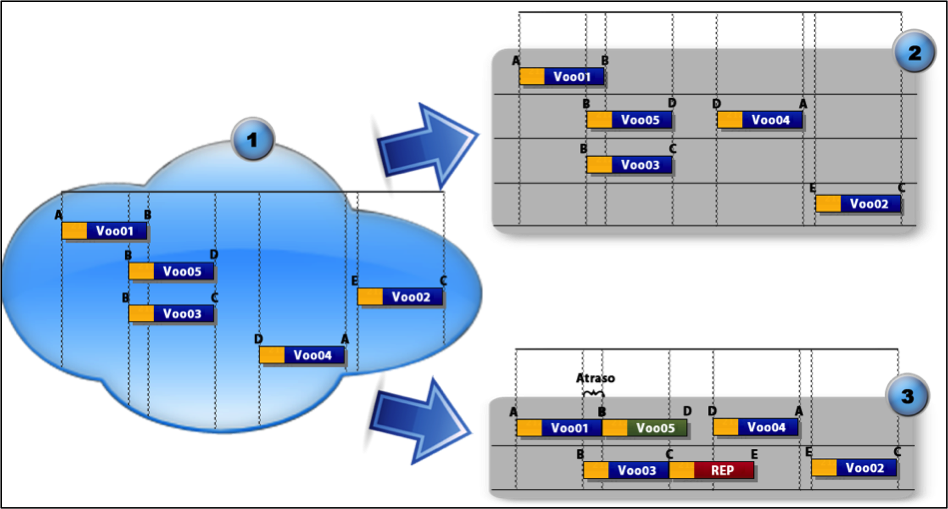
\includegraphics[scale=0.9]{./img/arpexample}
	\caption{Construção de Trilhos de Aeronaves}
	\label{fig:arpexample}
\end{figure}

A parte 1 da Figura \ref{fig:arpexample} representa os voos da companhia que ainda não foram cobertos por nenhuma aeronave e nas partes 2 e 3 são demonstrado duas formas de organizar esses voos em trilhos. 

	Na parte 2 temos a melhor forma possível de se organizar os voos da parte 1 utilizando apenas os arcos do tipo 1, ou seja sem a utilização de atrasos ou de voos de reposicionamento. Dessa forma se consegue uma formação com 4 trilhos.

	Na parte 3 temos a melhor forma de organizar os voos utilizando todos os arcos e um atraso máximo equivalente a um tempo de solo. Dessa forma se consegue uma formação com apenas 2 trilhos.

	Pode-se verificar que a utilização de diferentes tipos de arcos pode proporcionar uma melhora significativa  no número de trilhos. Porém essa abordagem faz com que o número de soluções possíveis tenha uma cardinalidade muito superior a utilização de arcos apenas do tipo 1 que por si só já gera uma quantidade de soluções bem elevada, por isso os arcos devem ser utilizados de forma controlada. 


  
%%%% Até aqui %%%%%%%%%%

\chapter{Método Proposto} \label{cap:metodoprop}
  
O método proposto se utiliza do GRASP, do ILS e da abordagem exata através da
programação linear inteira, pretendendo tirar proveito das vantagens de cada
uma dessas técnicas. Ou seja, combinando a agilidade dos métodos heurísticos com
a optimalidade do método exato.
  
Da mesma forma que em outras abordagens heurísticas, esse novo algoritmo
consome pouco tempo computacional, em relação ao método exato e tem a capacidade
de escapar de mínimos locais.
  
O GRASP foi utilizado como a base do algoritmo, onde a parte da construção
seguiu a sua definição padrão, com a geração de uma lista restrita de candidatos
(LRC) e a posterior escolha aleatória entre esses elementos. A parte da busca
local foi adaptada para executar em conjunto com o ILS modificado. Para o ILS
foram definidos algumas estruturas de vizinhança que foram utilizadas
na busca local, e a perturbação foi feita com a utilização de um \textit{solver}
em uma parte do problema. Essa abordagem permite que o algoritmo gere boas
soluções e escape de mínimos locais além de promover uma aceleração na obtenção
de boas soluções, pois quando o \textit{solver} encontra uma melhor solução ele
consegue mudar o espaço de soluções em que a busca era efetuada.


O \textit{solver} é utilizado para resolver um modelo matemático que foi
desenvolvido baseado na proposta de \cite{pontes2002} que é aplicado a uma parte do problema cada
vez que se deseja fazer uma perturbação. Enquanto a busca local usa o método de
descida, variando entre três estruturas de vizinhança, o \textit{swap-x}, o
\textit{crossover} e a \textit{compactação}. Mais adiante serão dado mais
detalhes sobre o modelo matemático, a forma de escolha do sub problema, da fase
de construção que foi implementada, da busca local e das implementações que não
tiveram êxito.

\section{Modelo matemático} \label{sec:modelomat}

   
A modelagem proposta por \cite{pontes2002} aborda todas as restrições do
problema fazendo com que a quantidade de restrições geradas seja muito elevada.
A idéia utilizada na nossa formulação é a de tentar reduzir ao máximo a
quantidade de restrições necessárias. Isso é feito com a modelagem de apenas
algumas restrições, aquelas que são possíveis no mundo real.

Primeiro se percebeu que não há necessidade de modelar os 4 tipos de arcos para
cada voo, uma vez que dados dois voos só pode vir a ocorrer dois tipos de arcos
possíveis entre eles. Essa situação é ilustrada na Figura
\ref{fig:modelagem_arcos}.

\begin{figure}[ht]
	\centering
	\caption{Arcos necessários para ligar dois voos. \newline \mbox{Fonte:
	(Própria)}}\label{fig:modelagem_arcos}
	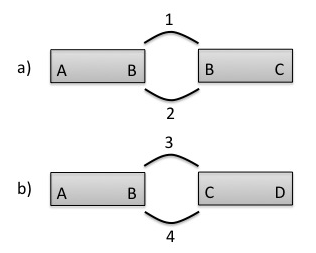
\includegraphics[scale=0.4]{./img/modelagem_arcos}
\end{figure}


Em a) os voos respeitam a restrição geográfica, dessa forma apenas os arcos de
tipo 1 e 2 precisam ser modelados uma vez que não teria sentido fazer um voo de
reposicionamento nessa situação. Em b) os aeroportos em questão são diferentes,
sendo necessário apenas a modelagem dos arcos do tipo 3 e 4, perceba que não
teria outra alternativa se não fazer um voo de reposicionamento.

\subsection{Definição}

Seja $D = (V,A)$ um grafo representando uma instância do PCTA, onde o conjunto
de vértice $V = {v_{i}:i \in I}$ de D é indexado por $I = {1, 2, ..., n+1,
n+2}$ onde $v_{n+1}$ e $v_{n+2}$, identificam, respectivamente, os nós fonte e
destino. E os nós restantes referem-se ao conjunto de nós originais, com $n$
elementos. Sejam os custos ${c_{ij}:(i,j) \in A}$ introduzidos acima, estando
associados com cada arco do grafo.
  
Seja ${x_{ij}:(i,j) \in A}$ um conjunto binário 0-1 de variáveis usada para
controlar a inclusão $(x_{ij} = 1)$ ou a exclusão $(x_{ij} = 0)$ de um arco
(possível conexão) entre vértices (voos) $v_{i}$ e $v_{j}$. O conjunto
$\overline{I}$ identifica o conjunto de nós excluindo o nó fonte $(v_{n+1})$ e
o nó de destino $(v_{n+2})$. A função objetivo foi dividida para facilitar o
entendimento de como é feito o custo de adicionar um trilho. Variáveis reais
$\delta_{i}$ e $\theta_{i}$, $i \in \overline{I}$ são usados para representar,
respectivamente, o desvio do tempo de partida sugerido e a norma desse desvio
para $v_{i}$. Essas variáveis devem no entanto obedecer $-\gamma_{i} \geq
\delta_{i} \geq \gamma_{i}$ e $0 \geq \theta_{i} \geq \gamma_{i}$, onde
$\gamma_{i}$ é o valor máximo de desvio permitido (em cada direção) do tempo de
partida sugerido para o voo. Finalmente o tempo de partida sugerido que é dado
por $s_{i}:i \in \overline{I}$.
  
\section{Função objetivo}

\begin{equation}
Minimizar \  \ \sum_{j \in \overline{I}} x_{v_{n+1}j}(CUSTO\_TRILHO) + \sum_{i \in
\overline{I}} \sum_{j \in I} x_{ij}c_{ij} + \sum_{i \in
\overline{I}} \theta_{i}
\end{equation}

\section{Restrições}

\begin{enumerate}


\item[a)] Garantia de recobrimento dos voos \\
\begin{equation}
  \sum_{i \in I} x_{ij}= 1 \   \ \forall_{j} \in \overline{I} 
\end{equation}
\begin{equation}
\sum_{j \in I} x_{ij} = 1 \   \ \forall_{i} \in \overline{I}
\end{equation}





\item[b)] Viabilidade das conexões \\
\begin{equation}
s_{i} + t_{i}x_{ij} - M(1 - x_{ij}) + \delta_{i} \leq s_{j} + \delta_{j} \   \ \forall_{i,j} \in \overline{I}
\end{equation}
%\begin{equation}
%\sum_{i \in I} x_{i(n+1)} = 0
%\end{equation}
%\begin{equation}
%\sum_{j \in I} x_{(n+2)j} = 0
%\end{equation}

\item[c)] Modulo do desvio do tempo de partida sugerido \\
\begin{equation}
\theta_{i} \geq \delta_{i} \   \ \forall_{i} \in \overline{I}
\end{equation}
\begin{equation}
\theta_{i} \geq -\delta_{i} \   \ \forall_{i} \in \overline{I}
\end{equation}

\item[d)] Limites das variáveis \\
\begin{equation}
-\gamma_{i} \geq \delta_{i} \geq \gamma_{i} \   \ \forall_{i} \in \overline{I}
\end{equation}
\begin{equation}
0 \geq \theta_{i} \geq \gamma_{i} \   \ \forall{i} \in \overline{I}
\end{equation}
\begin{equation}
x_{ij} \in \{0,1\}
\end{equation}
\end{enumerate}

\clearpage

Pode-se perceber que o modelo matemático não faz menção ao tempo de solo ($g$).
Isso ocorre pois esse tempo é incorporado ao voo como demonstrado na Figura
\ref{fig:conversion}, ou seja o tempo de partida sugerido $s$ passa a ter o
valor $s - g$ e a duração $t$ do voo passa a ter o valor $t + g$. Uma vantagem
de usar essa abordagem que integra o tempo de solo ao voo é a redução da
quantidade de restrições do problema.

\begin{figure}[ht]
	\caption{Conversão de um voo para ser utilizado no
	solver. \newline \mbox{Fonte: (Própria)}}\label{fig:conversion}
	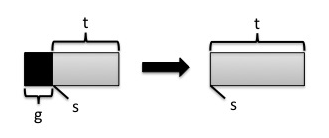
\includegraphics[scale=0.4]{./img/conversion}
	
\end{figure}

Além disso o conjunto $A$ contém apenas um tipo de arco, o arco do tipo 1 se os
voos satisfazem a restrição geográfica e o arco do tipo 3 caso não satisfaçam.
Os arcos dos tipos 2 e 4 são modelados a partir  da variável $\delta$ que tem
seu custo acrescentado na função objetivo.

Essa estratégia permite a redução de 3 arcos para cada voo, o que deixa o
modelo mais leve.

O calculo dos custos são feitos através de um pré-processamento, onde os arcos
viáveis recebem os valores referentes ao seu tipo, por exemplo, no caso de um
arco originário do nó origem, arco do tipo 6, um custo 1000 é atribuído. No
caso de arcos que deverão ser evitados um custo elevado é atribuído.
  	
  	
%\section{Pré-processmanto da instância}

%No caso da instância possuir mais de um dia de operação então pode-se quebra-la
%em dias se houver tempo vago entre os dias dessa instância.
  
\section{Fase de construção do GRASP}
  
A construção da solução é feita elemento a elemento utilizando o
GRASP. Inicialmente é feita a ordenação do conjunto de voos a partir do seu
tempo de partida sugerido. O algoritmo só termina quando todos os voos já
foram alocados em algum trilho.
  
Existem duas formas de fazer a montagem da solução, uma seria a montagem de
trilhos de forma sequencial, onde um novo trilho só é iniciado quando o anterior
se encontra saturado. A outra forma é a montagem de trilhos de forma paralela,
que, a priori, provocaria uma melhor distribuição dos voos. Na prática a
primeira abordagem foi adotada, pois, nas instâncias disponíveis ela apresentou,
sempre, soluções de melhor qualidade. 

Pode ser que para instâncias com alguma característica específica a
estratégia de montagem dos trilhos de forma paralela pode apresentar melhores
resultados.

\begin{figure}[h]
\caption{Pseudocódigo do procedimento de seleção de um voo inicial. \newline
\mbox{Fonte: Própria}}\label{alg:selectinit}
\begin{programma}
\ALGORITHM{selecionaVooInicial(V)}

\STATE $LCI$ \GETS cincoPrimeirosVoos($V$);
\STATE $h(v_{min}) \GETS min\{h(v) \mid v \in LCI\}$;
\STATE $h(v_{max}) \GETS max\{h(v) \mid v \in LCI\}$;
\STATE $LRI \GETS \{v \in LCI \mid h(v) \leq h(v_{min}) + \alpha(h(v_{max}) -
h(v_{min}))\}$;
\STATE Selecione aleatoriamente um elemento $v \in LRI$;
\STATE\RETURN $v$;
\ENDALGORITHM
\end{programma}
\end{figure}
  
\subsection{Formação dos trilhos de forma sequencial}

Quando se pensa na escolha do primeiro voo do trilho, a decisão imediata é a
escolha do voo que contenha o menor horário de partida sugerido, ou seja, o voo
mais próximo. Porém essa escolha reduz a quantidade de soluções que podem ser
geradas, isso ocorre pois o primeiro voo tem uma grande influência nas
possíveis soluções que um trilho pode assumir. Para evitar isso a escolha do
primeiro voo de um trilho é feita baseando-se nos 5 voos com menor horário de
partida que ainda não estejam alocados a nenhum outro trilho. 

Esses voos são adicionados a lista de candidatos iniciais (LCI) em seguida é
feita a escolha do elemento que irá iniciar o novo trilho levando em
consideração apenas os elementos que possuam o horário de partida distante de
até $\alpha \%$ do voo de menor horário de partida. Isso é feito para
evitar a escolha de um voo muito distante do menor voo.

\begin{figure}[h]
\caption{Pseudocódigo do procedimento de formação sequencial dos trilhos.
\newline
\mbox{Fonte: Própria}}\label{alg:formseq}
\begin{programma}
\ALGORITHM{construçãoSequencial(V)}

\STATE Ordene o conjunto de voos não alocados $V$;
\STATE $M \GETS \emptyset$;
\WHILE{$V \neq \emptyset$}
\STATE $v \GETS selecionaVooInicial(V)$
\STATE $T \GETS \{v\}$;
\STATE $T \GETS completaTrilho(T)$;
\STATE $V \GETS V - \{v \in T\}$;
\STATE $M \GETS M \cup T$;
\ENDWHILE
\STATE\RETURN $M$;

\ENDALGORITHM
\end{programma}
\end{figure}

\subsection{Formação dos trilhos de forma paralela}
 
Nessa estratégia um trilho é iniciado sempre que existe um voo que não pode ser
inserido em nenhum dos trilhos que estejam sendo montados, mantendo-se assim um
conjunto de trilhos disponíveis (CTD).

Em cada iteração o trilho corrente (TC) é escolhido a partir do CTD de forma
aleatória. Feito isso, adiciona-se um voo a esse trilho. Caso não existam voos
candidatos para adição no TC este é removido da CTD e uma nova iteração é
iniciada.

\begin{figure}[h]
\caption{Pseudocódigo do procedimento de formação paralela dos trilhos.
\newline
\mbox{Fonte: Própria}}\label{alg:formparalel}
\begin{programma}
\ALGORITHM{construçãoParalela(V)}

\STATE Ordene o conjunto de voos não alocados $V$;
\STATE $M \GETS \emptyset$;
\STATE $CTD \GETS \emptyset$;
\WHILE{$V \neq \emptyset$}
\STATE $v \GETS selecionaVooInicial(V)$
\IF {$v$ pode ser inserido em um trilho do CTD}
	\STATE $TC \GETS escolheTrilhoAleatório(CTD)$;
	\STATE $nv \GETS selecionaVooCandidato(TC)$;
	\IF {$nv = \emptyset$}
		\STATE $CDT \GETS CDT - \{TC\}$
		\STATE $M \GETS M \cup \{TC\}$
	\ELSE
		\STATE $TC \GETS TC \cup \{nv\}$
	\ENDIF
\ELSE
	\STATE $T \GETS \{v\}$; 
	\STATE $CTD \GETS CTD \cup T$ 	
\ENDIF
\ENDWHILE

\STATE $M = M \cup \{t \in CTD\}$;
\STATE\RETURN $M$;

\ENDALGORITHM
\end{programma}
\end{figure}

\begin{figure}[h]
\caption{Pseudocódigo de calculo do proximo voo de um trilho
\newline
\mbox{Fonte: Própria}}\label{alg:calcvoo}
\begin{programma}
\ALGORITHM{obtemProximoVoo(T,V)}

\STATE $A \GETS \{1,2,3,4\}$;
\STATE $a \GETS sorteaTipoDeArco(TiposDeArco, P_{1},P_{2},P_{3},P_{4})$;
\STATE $A \GETS A - \{a\}$;
\STATE $v \GETS ultimoVoo(T)$;

\FOR{$i$ \FROM $1$ \TO $4$}\PGlnlabel{forline}
\STATE $c \GETS proximoCandidato(v, V, a)$;
\IF {$c = \emptyset$}
	\STATE $a \GETS proximoArco(A)$;
	\STATE $A \GETS A - \{a\}$;
\ELSE
	\STATE\RETURN $c$;
\ENDIF 
\ENDFOR

\STATE\RETURN $\emptyset$;

\ENDALGORITHM
\end{programma}
\end{figure}
  
\subsection{Escolha dos voos de um trilho}

A escolha do primeiro voo de um trilho é feita como explicado nas seções
anteriores enquanto os demais voos são escolhidos tendo como base um tipo de
arco e uma lista restrita de candidatos (CLR).
 
Os tipos de arcos foram definidos no Capítulo \ref{cap:descprob}, porém nessa
etapa apenas 4 tipos são considerados, o   $A_{1},A_{2},A_{3},A_{4}$ que
representam formas de ligações entre os voos. Os arcos do tipo 5 e 6 só são
utilizados na modelagem matemática. Os arcos do tipo 1 permitem a
ligação de voos sem a utilização de atrasos e/ou reposicionamentos. Os arcos do
tipo 2 utilizam atrasos mas não o reposicionamento. Os arcos do tipo 3 permitem
o sequenciamento com a utilização de um voo de reposicionamento mas sem inserir
atraso em nenhum dos voos envolvidos. Os arcos do tipo 4 utilizam-se de atrasos
e de um voo de reposicionamento para fazer a ligação entre dois voos. Os arcos
do tipo 5 pargem do nó \textit{source} e servem para modelar o inicio de um
trilho. Os arcos do tipo 6 tem chegam ao nó \textit{sink} e indicam o fim de um
trilho.

Primeiramente é feita a escolha do tipo de arco que será utilizado para efetuar
a ligação do ultimo voo do trilho corrente. Essa escolha é feita tendo
como base as probabilidades de cada um desses arcos acontecer. Essa
probabilidade foi definida como sendo
$P(A_{1})=0.79,P(A_{2})=0.16,P(A_{3})=0.04,P(A_{4})=0.01$ pois a solução ótima
do problema real da Rio Sul apresentava essas características. Esses valores
são empíricos e para determinadas instâncias podem gerar melhores soluções se
alterados.

De posse do tipo de arco, é feita então a formação da lista de candidatos. Essa
lista é ordenada de acordo com o seu horário de partida sugerido, caso o arco
seja do tipo $A_{1}$, ou pelo custo associado a sua escolha para os demais
tipos de arco. No caso da lista de candidatos não possuir nenhum voo, então
outro tipo de arco é sorteado, até que não seja possível acrescentar voos ao
trilho de nenhuma forma, quando isso ocorrer a construção
desse trilho é finalizada.
 
Caso seja possível a obtenção de uma lista de candidatos então ela é reduzida
tendo como base o passo 4 a 6 do algoritmo \ref{alg:graspcons} formando assim a
lista de candidatos restrita (LCR), essa redução remove os candidatos que estão
muito afastado do melhor candidato da lista. Como está lista se encontra
ordenada, então, o elemento de menor impacto ($v_{menor}$) na solução é o
primeiro e o de maior impacto ($v_{maior}$) é o último. A LCR contém os
candidatos que tenha o valor de impacto na solução de até $valor_{menor} +
\alpha*(valor_{maior} + valor_{menor})$, onde $\alpha$ é o grau de
gulosidade do GRASP. O candidato deve ser escolhido de forma aleatória entre os
elementos da LCR.
 
 \section{Fase de busca local do GRASP}

Com a finalização da etapa anterior tem-se uma solução do problema. A fase de busca
local efetua modificações nessa solução com a finalidade de obter outras
melhores que estejam próximos a ela, isso é feito através da aplicação das
estruturas de vizinhanças. No método proposto essa fase foi implementada através
da utilização da metaheurística ILS que alterna busca local com pertubações
conseguindo assim escapar de mínimos locais quando não consegue mais melhorar a
solução, ou seja, primeiro são aplicados as estruturas de vizinhança, visando
obter o valor ótimo local da solução, depois é feita uma perturbação que
diversifica melhorando o valor da função objetivo através da aplicação do
modelo matemático que foi desenvolvido em uma parte do problema. Quando nenhuma
das duas estratégias consegue melhorar a solução então a busca local encerra e
uma nova iteração do GRASP pode ser iniciada.
 
\subsection{Estruturas de vizinhança}
 
Foram definidas três estruturas de vizinhança para serem utilizadas na busca
local, o Swap-X e o Cross-Over, que tem o objetivo de remover modificações nos
horários de partida sugeridos dos voos, e a Compactação, que promove a redução
do número de trilhos. Abaixo essa estruturas são explicadas.
 
\subsubsection{Swap-X}

Esse operador efetua a troca de X voos de um trilho por um conjunto de voos de
outro trilho. Dessa forma pode-se conseguir remover os atrasos que foram criados
na etapa de construção. No método proposto apenas os movimentos do tipo Swap-1
e Swap-2 são utilizados, pois essa vizinhança é considerada grande. Na Figura
\ref{fig:swap1} um caso de melhoria no custo dos trilhos é exemplificada.

\begin{figure}[ht]
	\caption{Estrutura de vizinhança Swap-1. \newline \mbox{Fonte:
	(Própria)}}\label{fig:swap1}
	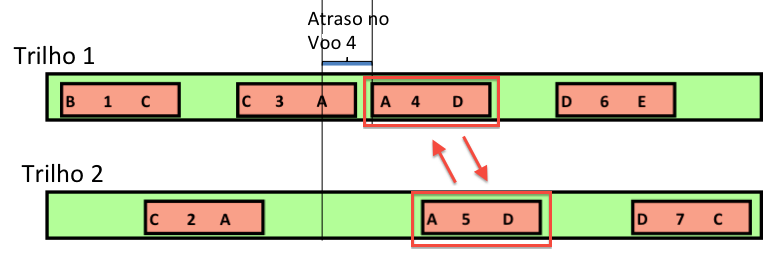
\includegraphics[scale=0.4]{./img/swap-1}
	
\end{figure}
 
 \subsubsection{Cross-Over}
 
A ideia do operador $crossover$ é a de efetuar troca entre dois segmentos de
trilhos com a finalidade de gerar novos trilhos com menos modificações no
horário de partida. A Figura \ref{fig:crossover} ilustra uma melhoria causada por um
movimento desse tipo.


\begin{figure}[ht]
	\caption{Estrutura de vizinhança CrossOver. \newline \mbox{Fonte:
	(Própria)}}\label{fig:crossover}
	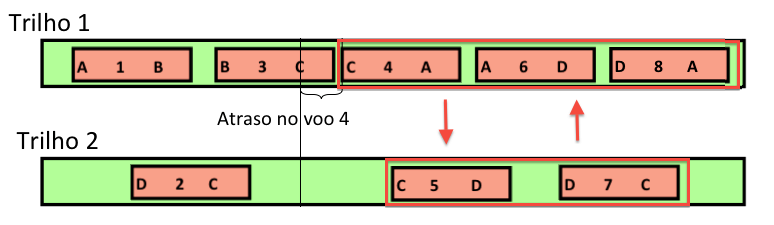
\includegraphics[scale=0.4]{./img/crossover}
	
\end{figure}
 
 \subsubsection{Compactação}
 
A compactação é a única estrutura de vizinhança utilizada que é capaz de
reduzir a quantidade de trilhos da solução final.
 
Isso ocorre porque ela consegue, insere um trilho em outro de forma direta ou
com a utilização de um voo de reposicionamento.
 
A figura \ref{fig:compactacao} mostra a redução de um trilho com a utilização
desse movimento.

\begin{figure}[ht] 
	\caption{Estrutura de vizinhança Compactação. \newline \mbox{Fonte:
	(Própria)}}\label{fig:compactacao}
	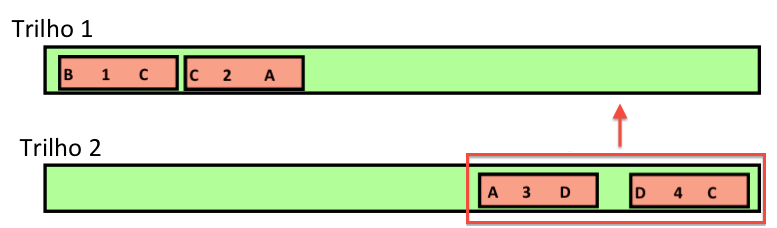
\includegraphics[scale=0.4]{./img/compactacao}
	
\end{figure}
 
 \subsection{Perturbação usando o método exato}
   
A perturbação normalmente é utilizada quando as estruturas de vizinhança não
conseguem melhorar a solução, quando isso ocorre, pode-se dizer que a
solução corrente é a ótima local com relação a vizinhança que foi definida.
 
Para tentar encontrar outros mínimos locais aplica-se uma modificação na
estrutura da solução, mesmo que isso provoque uma piora na sua qualidade. Isso
se mostra interessante para o algoritmo pois ele irá efetuar busca de melhorias
em outros locais no espaço de soluções através da sua busca local.
 
O método de perturbação utilizado aqui difere do que normalmente é aplicado
pois a solução tem a sua estrutura modificada e ainda consegue melhorar a sua
qualidade. Isso é feito através da aplicação do modelo matemático em uma
parte do problema. A sua utilização ocorre com a seleção de um conjunto de
trilhos, e sua a posterior aplicação no solver com o modelo desenvolvido
configurado para o conjunto de voos da seleção.

O método exato retorna a configuração ótima desses voos, que
são agrupados novamente a solução antiga. O solver tem um tempo máximo
estabelecido e se não retornar nenhuma solução considera-se que não houve
melhora sua aplicação.

A seleção dos trilhos é feita com base no seu
\textit{grau de compactação} que é definido como sendo porcentagem de
utilização efetiva de um trilho com relação ao tempo de partida do primeiro voo
e o tempo de chegada do último voo da instância, ou seja, quanto maior o tempo
que a aeronave, que opera um determinado trilho, permanece voando maior será o
seu grau de compactação. O calculo do grau de compactação não leva em
consideração os voos de reposicionamento, pois eles não estão no planejamento
inicial e por sua vez não são passados para o modelo.

Existe três formas de fazer a seleção dos trilhos que serão aplicados no solver,
pode-se adicionar os trilhos que possuem o maior grau de compactação, pode-se
adicionar os trilhos que possuem o menor grau de compactação ou pode-se alternar
entre a escolha de um trilho com o maior grau de compactação e um de menor grau
de compactação.

Na prática adotou-se a segunda abordagem, selecionando os trilhos de menor grau
de compactação, pois os resultados foram melhores.
 
Os trilhos são adicionados a solução até o limite de 80 voos, pois o solver
conseguiu em nossos experimentos resolver um problema desse porte de forma
imediata. 


 
   
  \chapter{Resultados preliminares e discursões}

Todos os algoritmos descritos foram desenvolvidas na linguagem C++ usando a biblioteca CPLEX Academic 12 para implementar o mecanismo de programação inteira. Todos os experimentos computacionais foram feitos em um notebook com a seguinte especificação: Pentium T4500 2.3 Ghz com 2 GB de RAM e rodando o sistema operacional sistema operacional Linux Ubuntu 11.04.

Foram efetuadas 10 iterações do GRASP usando um $\alpha$ de 0.5 e a busca local finalizava quando não conseguia melhorar o resultado. Para demonstrar a eficiência dos resultados foram realizadas comparações com o resultado ótimo obtido com um procedimento de programação inteira implementando o modelo descrito no capítulo \ref{cap:descprob}. A coluna $s*$ indica o valor ótimo. O método híbrido foi executado 20 vezes e apenas a média dos valores obtidos foram levados em consideração. A coluna $s$ indica a média dos valores obtidos com a execução do algoritmo, a coluna tempo indica a média da duração das execuções em segundos. A coluna final indicada por $GAP$ indica a diferença percentual das soluções e é calculado como segue:

\[  GAP = (s* - s)/s \]

Para os testes foram utilizados duas instâncias diárias, uma da Rio-Sul(107 voos) e outra da TAM (241 voos).  Com a finalidade de permitir estimar o tempo computacional necessário para resolver instâncias maiores foi proposto a extensão da frequência dos voos da instância Rio-Sul para uma semana, dessa forma foi gerado uma instância com 749 voos. Para simplificar foram adotados o tempo de solo de 20 minutos para todos os aeroportos.

A resolução dessas instâncias foram parametrizadas levando em consideração dois cenários. O cenário 1 faz o sequênciamento dos voos sem a permissão de utilizar nenhum atraso, essa representação é comum nas companhias que não aceitam a modificação do planejamento inicial. O cenário 2 se utiliza de atrasos permitindo assim uma maior liberdade na hora da montagem dos trilhos. Os parâmetros utilizados são detalhados na Tabela \ref{tab:params}.

\begin{table}
\caption{Parametrização dos cenários}\label{tab:params}
\begin{center}


\begin{tabular}{l|rr}
\hline

 & Cenário 1 & Cenário 2 \\
 \hline
 Atraso Maximo & 0 & 10 \\
 Prob. Arc. Tipo 1 & 0.92 & 0.69\\ 
 Prob. Arc. Tipo 2 & 0 & 0.16\\
 Prob. Arc. Tipo 3 & 0.08 & 0.04 \\
 Prob. Arc. Tipo 4 & 0 & 0.01 \\
  
\hline

\end{tabular}
\end{center}
\end{table}

 
%A Tabela \ref{tab:cenario1} e \ref{tab:cenario2} mostram os resultados as melhores soluções obtidas. No caso dos problemas diários e da instância da Rio Sul estendida a utilização do solver é suficiente e retorna o resultado ótimo em um tempo totalmente aceitável, dessa forma o método está sendo desenvolvido parar a resolução de problemas de grande porte. No caso de problemas reais isso iria refletir nas frotas mais comuns das companhias aéreas, que é onde se encontra a maior demanda de passageiros. Caso alguma informação extra seja necessária os anexos \ref{anx:netriosul} a \ref{anx:resulttam} apresentam a descrição completa das instâncias e das soluções que foram obtidas, 


%Rio Sul & 17.138 & 17 & 0 & 2 & XX & XX & 0\\
%TAM & 35.334 & 34 & 0 & 10 & XX & XX & 0 \\
%Rio Sul Estendida & 18392 & 17 & 0 & 20 & XX & XX & 0\\
%TAM Estendida & XX & XX & XX & XX & XX & XX & XX \\

\begin{table}[ht]
\caption{Resultados do cenário 1}\label{tab:cenario1}
\begin{center}


\begin{tabular}{l r r r r}
\hline

Instância & BKS & Resultado & Tempo(s) & GAP \\
\hline

Rio Sul & 17.138 & 17.138 & 4.8 & 0\\
TAM & 35.334 & 35.348 & 37 &  0.0004\\
Rio Sul Estendida & 18.392 & 21.911 & 525 & 0.19\\
%TAM Estendida & XX & XX & XX & XX \\

\hline
\end{tabular}

\end{center}
\end{table}

\begin{table}[ht]
\caption{Resultados do cenário 2}\label{tab:cenario2}
\begin{center}


\begin{tabular}{l r r r r}
\hline

Instância & BKS & Resultado & Tempo(s) & GAP \\
\hline

Rio Sul & 16.158 & 16.158 & 5 & 0\\
TAM & 35.015 & 35015 & 22 & 0 \\
Rio Sul Estendida & 17.433 & 20564 & 494 & 0.18\\ 
%TAM Estendida & XX & XX & XX & XX \\

\hline
\end{tabular}

\end{center}
\end{table}

	Pode-se observar que nos dois cenários a solução ótima foi obtida para a instância da Rio-Sul. Na instância da TAM a solução ótima foi encontrada, porém, na média o cenário 1 encontrou uma solução bem próxima. Essas duas instâncias representam um horizonte de tempo de um dia. Na instância da Rio-Sul estendida que representam uma semana de operação as soluções ficaram em média 0.19 do ótimo para o cenário 1 e 0.18 no cenário 2 com um tempo aproximado de 8 minutos. Para o procedimento programação linear não foram inseridos limites previamente calculados, de modo que a ferramenta utilizou apenas a relaxação linear.
  
 Alguns ajustes ainda podem melhorar o modelo híbrido para que ele possa se aproximar mais da solução ótima. A modificação da estrutura a ser otimizada na busca local pode ser um ponto que ajude a melhorar os resultados, pois a literatura mostra que esse é um dos pontos mais importantes de uma heurística híbrida.
 
 Uma das grandes dificuldades encontradas no trabalho foi a falta de instâncias na literatura tornando difícil a comparação de resultados com outras abordagens. Com isso existe a necessidade de geração de um conjunto de instâncias e a sua publicação para fins comparativos.
 
 Existe ainda a possibilidade de uma implementação paralela que ainda está em fase de planejamento e que se demonstrar resultados interessantes em tempo hábil será adicionada a dissertação.
 

%Com a eficiência obtida com o método exato existe uma necessidade de geração de instâncias maiores que possam ser utilizadas parar ajustar e justificar a utilização de uma abordagem mais complexa como o uso de uma metaheurística híbrida.

%Atualmente o método híbrido conseguiu resolver a instância \textit{TAM Estendida} com o tempo de 60s e Custo total de 43344, que parece %ser uma boa solução tendo como base os resultados obtidos com a instância que lhe serviu de base.

%Atualmente existe a necessidade de um melhor ajuste no método híbrido para que ele possa conseguir resultados mais robustos.

%A utilização de uma abordagem exata em conjunto com metaheurísticas está sendo cada vez mais utilizado na literatura. Porém a escolha da estrutura a ser otimizada deve ser bem escolhida para não aumentar demasiadamente a capacidade computacional necessária para resolver o problema.



%Para demonstrar a eficiência em termos de qualidade da solução da metaheurística GILS, realizamos comparações com um  procedimento exato B&B (XPRESS MP, 2004), implementando o modelo STSP apresentado por Lee (1996). Para cada instância da Tabela 1 temos as duas primeiras colunas representando as dimensões das instâncias testadas e as colunas restantes divididas em dois grupos: procedimento B&B e GILS. No caso do procedimento B&B, a coluna z* indica o valor ótimo e a coluna tempo indica o tempo computacional, em segundos, gasto na resolução da instância. Já para o grupo da metaheurística GILS as colunas adicionais, além da coluna tempo, são: iter que indica a iteração onde foi encontrada melhor solução, z que indica o valor obtido pelo GILS e, Δ (gap) que indica a diferença percentual entre as soluções:
%Δ = [ (z – z*) / z* ] x 100.


% % \chapter{Conclusões}
  
  %Os resultados obtidos, apesar de iniciais, indicam que existe um grande potencial na utilização desse conjunto de técnicas. O que ainda %é necessário é a construção ou a obtenção de uma maior quantidade de instâncias para permitir explorar e ajustar melhor diversos pontos do %método proposto.
  
 % A utilização de uma abordagem exata em conjunto com metaheurísticas está sendo cada vez mais utilizado na literatura. Porém a escolha da %estrutura a ser otimizada deve ser bem escolhida para não aumentar demasiadamente a capacidade computacional necessária para resolver o %problema.


 
% Bibliografia o arquivo


\bibliographystyle{abnt-alf} % Estilo autor-data
\bibliography{bibliografia}    % As referencias deste testo est?o no arquivo modelotese.bib
\ABNTaddcontentsline{toc}{chapter}{Refer?ncias bibliogr?ficas}


\anexo

\chapter{Rede de voos da Rio-Sul}\label{anx:netriosul}

A rede de voos abaixo está organizada em 8 colunas que representam
respectivamente:

\begin{itemize}
  \item Número do voo: Sequência que representa a posição do voo na lista.
  \item Nome do voo: Nome que identifica o voo junto a companhia aérea.
  \item Dia de partida do voo: Representa em que dia o voo irá partir. O dia
  0 (zero) representa o primeiro dia de operação do planejamento. Cada dia
  acrescentado acrescenta 24 horas ao horário de partida do voo.
  \item Horário de partida do voo: Identifica em que horário o voo irá partir.
  \item Dia de chegada do voo: Representa em que dia o voo irá chegar. O dia
  0 (zero) representa o primeiro dia de operação do planejamento. Cada dia
  acrescentado acrescenta 24 horas ao horário de chegada do voo.
  \item Horário de chegada do voo: Identifica em que horário o voo irá chegar.
  \item Aeroporto de partida: Identifica o aeroporto de partida do voo.
  \item Aeroporto de chegada: Identifica o aeroporto de chegada do voo.
    
\end{itemize}


\begin{scriptsize}

\begin{longtable}{l c c l}
001 SL166  0 08:00 0 08:31 GYN BSB & & & 055 SL598  0 16:00 0 17:55 CGH POA \\

002 SL155  0 08:32 0 10:33 GYN CGH & & & 056 SL568  0 16:02 0 17:03 CGH PLU \\

003 SL330  0 08:34 0 09:59 CGH VIX & & & 057 SL403  0 16:08 0 17:59 POA CGH \\

004 SL595  0 08:40 0 11:11 POA CGH & & & 058 SL273  0 16:10 0 17:51 SJP CGH \\

005 SL596  0 08:44 0 10:39 CGH POA & & & 059 SL391  0 16:12 0 17:55 FLN CGH \\

006 SL533  0 08:50 0 10:01 BSB PLU & & & 060 JH343  0 16:12 0 18:57 SSA CGH \\

007 SL280  0 08:52 0 09:43 CGH CWB & & & 061 SL481  0 17:00 0 17:45 CGH SDU \\

008 SL587  0 09:00 0 10:01 PLU CGH & & & 062 JH506  0 17:02 0 18:33 CGH BSB \\

009 SL520  0 09:02 0 09:47 SDU PLU & & & 063 SL405  0 17:14 0 19:57 CGH CGH \\

010 JH559  0 09:04 0 10:35 BSB CGH & & & 064 SL569  0 17:32 0 18:33 PLU CGH \\

011 SL406  0 09:06 0 09:55 SDU CGH & & & 065 SL152  0 17:44 0 19:35 CGH GYN \\

012 SL419  0 09:16 0 11:03 FLN CGH & & & 066 JH546  0 17:56 0 19:27 CGH BSB \\

013 SL542  0 09:28 0 10:31 CGH PLU & & & 067 SL572  0 17:58 0 18:59 CGH PLU \\

014 SL408  0 09:30 0 10:21 SDU CGH & & & 068 SL482  0 18:30 0 19:21 SDU CGH \\

015 JH345  0 09:30 0 12:23 SSA CGH & & & 069 JH341  0 18:50 1 00:19 JPA CGH \\

016 SL589  0 09:58 0 11:01 PLU CGH & & & 070 SL592  0 18:54 0 20:45 CGH POA \\

017 JH502  0 10:02 0 11:33 CGH BSB & & & 071 JH507  0 19:00 0 20:31 BSB CGH \\

018 SL281  0 10:08 0 10:59 CWB CGH & & & 072 SL528  0 19:02 0 19:47 SDU PLU \\

019 SL521  0 10:16 0 11:01 PLU SDU & & & 073 JH550  0 19:04 0 20:35 CGH BSB \\

020 SL532  0 10:20 0 11:31 PLU BSB & & & 074 SL537  0 19:22 0 20:33 BSB PLU \\

021 SL510  0 10:22 0 11:13 CGH CWB & & & 075 SL576  0 19:26 0 20:27 CGH PLU \\

022 SL544  0 10:32 0 11:33 CGH PLU & & & 076 SL573  0 19:34 0 20:35 PLU CGH \\

023 SL331  0 10:40 0 12:11 VIX CGH & & & 077 SL599  0 19:46 0 21:41 POA CGH \\

024 SL409  0 11:00 0 11:49 CGH SDU & & & 078 JH547  0 20:00 0 21:31 BSB CGH \\

025 SL543  0 11:00 0 12:03 PLU CGH & & & 079 SL153  0 20:04 0 22:05 GYN CGH \\

026 SL590  0 11:06 0 12:44 CGH POA & & & 080 SL483  0 20:08 0 20:53 CGH SDU \\

027 SL336  0 11:16 0 15:05 CGH REC & & & 081 SL412  0 20:10 0 21:29 CGH FLN \\

028 SL597  0 11:30 0 13:27 POA CGH & & & 082 SL529  0 20:14 0 20:59 PLU SDU \\

029 SL522  0 11:32 0 12:17 SDU PLU & & & 083 SL584  0 20:26 0 21:27 CGH PLU \\

030 SL150  0 11:42 0 13:33 CGH GYN & & & 084 SL514  0 20:30 0 21:21 CGH CWB \\

031 SL511  0 11:50 0 12:41 CWB CGH & & & 085 JH344  0 20:48 0 23:39 CGH SSA \\

032 JH503  0 12:02 0 13:33 BSB CGH & & & 086 SL577  0 21:02 0 22:03 PLU CGH \\

033 SL545  0 12:04 0 13:05 PLU CGH & & & 087 SL536  0 21:04 0 22:13 PLU BSB \\

034 SL470  0 12:28 0 13:19 SDU CGH & & & 088 JH551  0 21:04 0 22:35 BSB CGH \\

035 SL523  0 12:46 0 13:31 PLU SDU & & & 089 SL332  0 21:20 0 22:31 CGH VIX \\

036 JH342  0 13:00 0 15:45 CGH SSA & & & 090 SL492  0 21:30 0 22:21 SDU CGH \\

037 JH500  0 13:02 0 14:33 CGH BSB & & & 091 SL586  0 21:30 0 22:31 CGH PLU \\

038 SL147  0 13:10 0 18:03 BSB BSB & & & 092 SL530  0 21:34 0 22:19 SDU PLU \\

039 JH340  0 13:22 0 18:25 CGH JPA & & & 093 SL515  0 21:45 0 22:37 CWB CGH \\

040 SL591  0 13:30 0 14:57 POA CGH & & & 094 SL593  0 21:52 0 23:19 POA CGH \\

041 SL402  0 13:38 0 15:33 CGH POA & & & 095 SL585  0 22:04 0 23:05 PLU CGH \\

042 SL471  0 13:54 0 14:39 CGH SDU & & & 096 SL518  0 22:16 0 23:07 CGH CWB \\

043 SL390  0 13:56 0 15:41 CGH FLN & & & 097 SL413  0 22:22 0 23:31 FLN CGH \\

044 SL564  0 13:58 0 14:59 CGH PLU & & & 098 SL407  0 22:24 0 23:09 CGH SDU \\

045 SL151  0 13:58 0 15:59 GYN CGH & & & 099 SL167  0 22:42 0 23:13 BSB GYN \\

046 SL563  0 14:00 0 15:01 PLU CGH & & & 100 SL531  0 22:48 0 23:33 PLU SDU \\

047 SL272  0 14:12 0 15:51 CGH SJP & & & 101 JH558  0 22:56 1 00:27 CGH BSB \\

048 SL282  0 14:22 0 15:13 CGH CWB & & & 102 SL493  0 23:02 0 23:47 CGH SDU \\

049 SL508  0 14:56 0 15:41 SDU PLU & & & 103 SL333  0 23:04 1 00:15 VIX CGH \\

050 JH501  0 14:58 0 16:29 BSB CGH & & & 104 SL588  0 23:06 1 00:07 CGH PLU \\

051 SL480  0 15:30 0 16:21 SDU CGH & & & 105 SL594  0 23:18 1 01:57 CGH POA \\

052 SL283  0 15:42 0 16:37 CWB CGH & & & 106 SL154  0 23:22 1 01:13 CGH GYN \\

053 SL337  0 15:46 0 19:29 REC CGH & & & 107 SL418  0 23:32 1 01:19 CGH FLN \\

054 SL347  0 16:00 0 16:45 PLU SDU & & & \\

\end{longtable}

\end{scriptsize}
\chapter{Tempo dos voos da Rio-Sul}\label{anx:timeriosul}

A tabela abaixo está organizada em 3 colunas onde as duas primeiras representam
dois aeroportos distintos e a terceira representa o tempo de voo em minutos
entre esses dois aeroportos.

\begin{scriptsize}

\begin{longtable}{l l l l}


BSB CGH 0091 & CGH SJP 0049 & FLN SSA 0225 & PLU SDU 0045 \\
BSB CWB 0125 & CGH SSA 0171 & FLN VIX 0136 & PLU SJP 0067 \\
BSB FLN 0152 & CGH VIX 0087 & GYN JPA 0216 & PLU SSA 0113 \\
BSB GYN 0031 & CWB FLN 0028 & GYN PLU 0076 & PLU VIX 0044 \\
BSB JPA 0197 & CWB GYN 0114 & GYN POA 0173 & POA REC 0342 \\
BSB PLU 0071 & CWB JPA 0293 & GYN REC 0210 & POA SDU 0129 \\
BSB POA 0185 & CWB PLU 0095 & GYN SDU 0109 & POA SJP 0119 \\
BSB REC 0191 & CWB POA 0062 & GYN SJP 0054 & POA SSA 0267 \\
BSB SDU 0107 & CWB REC 0283 & GYN SSA 0143 & POA VIX 0177 \\
BSB SJP 0066 & CWB SDU 0078 & GYN VIX 0118 & REC SDU 0215 \\
BSB SSA 0125 & CWB SJP 0060 & JPA PLU 0198 & REC SJP 0242 \\
BSB VIX 0109 & CWB SSA 0208 & JPA POA 0352 & REC SSA 0075 \\
CGH CWB 0051 & CWB VIX 0125 & JPA REC 0013 & REC VIX 0169 \\
CGH FLN 0105 & FLN GYN 0142 & JPA SDU 0226 & SDU SJP 0079 \\
CGH GYN 0095 & FLN JPA 0311 & JPA SJP 0251 & SDU SSA 0130 \\
CGH JPA 0255 & FLN PLU 0114 & JPA SSA 0085 & SDU VIX 0048 \\
CGH PLU 0058 & FLN POA 0042 & JPA VIX 0181 & SJP SSA 0169 \\
CGH POA 0097 & FLN REC 0300 & PLU POA 0155 & SJP VIX 0110 \\
CGH REC 0246 & FLN SDU 0087 & PLU REC 0187 & SSA VIX 0097 \\
CGH SDU 0049 & FLN SJP 0088 & & \\


\end{longtable}

\end{scriptsize}
\chapter{Resultado ótimo da instância Rio-Sul}\label{anx:resultriosul}

O resultado está organizado em vários blocos que representam as rotas que foram
obtidas. Cada bloco inicia com um número que identifica a ordem em que a rota se
encontra na lista, seguido de um número que identifica a quantidade de voos
presentes nesta rota. Em seguida é descrito cada voo da rota seguindo o mesmo
padrão utilizado na descrição da instância. Os voos de reposicionamento se
encontram destacados em itálico.

Valor da função objetivo: 16158

\begin{scriptsize}

\begin{longtable}{l l l}

Rota[01 - 9]  & Rota[02 - 7]  & Rota[03 - 9] \\
SL166  0 08:00 0 08:31 GYN BSB & SL155  0 08:32 0 10:33 GYN CGH & SL330  0 08:34 0 09:59 CGH VIX\\
JH559  0 09:04 0 10:35 BSB CGH & SL590  0 11:06 0 12:44 CGH POA & SL331  0 10:40 0 12:11 VIX CGH\\
SL409  0 11:00 0 11:49 CGH SDU & SL591  0 13:30 0 14:57 POA CGH & \textit{REPO}
0 12:31 0 13:29 CGH PLU\\ 
SL470  0 12:28 0 13:19 SDU CGH & SL572  0 17:58 0 18:59 CGH PLU & SL563  0 14:00 0 15:01 PLU CGH\\
SL272  0 14:12 0 15:51 CGH SJP & SL573  0 19:34 0 20:35 PLU CGH & SL568  0 16:02 0 17:03 CGH PLU\\
SL273  0 16:10 0 17:51 SJP CGH(+1) & SL332  0 21:20 0 22:31 CGH VIX & SL569  0
17:32 0 18:33 PLU CGH\\ SL584  0 20:26 0 21:27 CGH PLU & SL333  0 23:04 1 00:15 VIX CGH & JH550  0 19:04 0 20:35 CGH BSB\\
SL585  0 22:04 0 23:05 PLU CGH & JH551  0 21:04 0 22:35 BSB CGH\\
SL418  0 23:32 1 01:19 CGH FLN & SL154  0 23:22 1 01:13 CGH GYN\\

\\

Rota[04 - 6]  & Rota[05 - 5]  & Rota[06 - 7] \\
SL595  0 08:40 0 11:11 POA CGH & SL596  0 08:44 0 10:39 CGH POA & SL533  0 08:50
0 10:01 BSB PLU (-1)\\
JH342  0 13:00 0 15:45 CGH SSA & SL597  0 11:30 0 13:27
POA CGH & SL532  0 10:20 0 11:31 PLU BSB\\ JH343  0 16:12 0 18:57 SSA CGH & SL598  0 16:00 0 17:55 CGH POA & JH503  0 12:02 0 13:33 BSB CGH\\
SL576  0 19:26 0 20:27 CGH PLU & SL599  0 19:46 0 21:41 POA CGH & SL282  0 14:22 0 15:13 CGH CWB\\
SL577  0 21:02 0 22:03 PLU CGH & SL407  0 22:24 0 23:09 CGH SDU & SL283  0 15:42 0 16:37 CWB CGH\\
JH558  0 22:56 1 00:27 CGH BSB & & SL405  0 17:14 0 19:57 CGH CGH\\
 &  & JH344  0 20:48 0 23:39 CGH SSA\\
 
\\

Rota[07 - 7]  & Rota[08 - 7]  & Rota[09 - 9] \\
SL280  0 08:52 0 09:43 CGH CWB & SL587  0 09:00 0 10:01 PLU CGH & SL520  0 09:02 0 09:47 SDU PLU\\
SL281  0 10:08 0 10:59 CWB CGH & SL510  0 10:22 0 11:13 CGH CWB & SL521  0 10:16 0 11:01 PLU SDU\\
SL564  0 13:58 0 14:59 CGH PLU & SL511  0 11:50 0 12:41 CWB CGH & SL522  0 11:32 0 12:17 SDU PLU\\
SL347  0 16:00 0 16:45 PLU SDU & SL390  0 13:56 0 15:41 CGH FLN & SL523  0 12:46 0 13:31 PLU SDU\\
SL482  0 18:30 0 19:21 SDU CGH & SL391  0 16:12 0 17:55 FLN CGH & SL508  0 14:56 0 15:41 SDU PLU\\
SL412  0 20:10 0 21:29 CGH FLN & SL592  0 18:54 0 20:45 CGH POA & \textit{REPO}  
0 16:01 0 16:59 PLU CGH\\ 
SL413  0 22:22 0 23:31 FLN CGH & SL593  0 21:52 0 23:19 POA CGH & SL152  0 17:44 0 19:35 CGH GYN\\
 &  & SL153  0 20:04 0 22:05 GYN CGH\\
 &  & SL588  0 23:06 1 00:07 CGH PLU\\

\\

Rota[10 - 10]  & Rota[11 - 6]  & Rota[12 - 7] \\
SL406  0 09:06 0 09:55 SDU CGH & SL419  0 09:16 0 11:03 FLN CGH & SL542  0 09:28 0 10:31 CGH PLU\\
SL544  0 10:32 0 11:33 CGH PLU & SL150  0 11:42 0 13:33 CGH GYN & SL543  0 11:00 0 12:03 PLU CGH\\
SL545  0 12:04 0 13:05 PLU CGH & SL151  0 13:58 0 15:59 GYN CGH & SL402  0 13:38 0 15:33 CGH POA\\
SL471  0 13:54 0 14:39 CGH SDU & JH546  0 17:56 0 19:27 CGH BSB & SL403  0 16:08 0 17:59 POA CGH\\
SL480  0 15:30 0 16:21 SDU CGH & JH547  0 20:00 0 21:31 BSB CGH & SL514  0 20:30 0 21:21 CGH CWB\\
SL481  0 17:00 0 17:45 CGH SDU & SL518  0 22:16 0 23:07 CGH CWB & SL515  0 21:45 0 22:37 CWB CGH\\
SL528  0 19:02 0 19:47 SDU PLU & & SL594  0 23:18 1 01:57 CGH POA\\
SL529  0 20:14 0 20:59 PLU SDU\\
SL492  0 21:30 0 22:21 SDU CGH\\
SL493  0 23:02 0 23:47 CGH SDU\\

\\

Rota[13 - 6]  & Rota[14 - 6]  & Rota[15 - 3] \\
SL408  0 09:30 0 10:21 SDU CGH & JH345  0 09:30 0 12:23 SSA CGH & SL589  0 09:58 0 11:01 PLU CGH\\
SL336  0 11:16 0 15:05 CGH REC & JH500  0 13:02 0 14:33 CGH BSB & JH340  0 13:22 0 18:25 CGH JPA\\
SL337  0 15:46 0 19:29 REC CGH & JH501  0 14:58 0 16:29 BSB CGH & JH341  0 18:50 1 00:19 JPA CGH\\
SL483  0 20:08 0 20:53 CGH SDU & JH506  0 17:02 0 18:33 CGH BSB\\
SL530  0 21:34 0 22:19 SDU PLU & JH507  0 19:00 0 20:31 BSB CGH\\
SL531  0 22:48 0 23:33 PLU SDU & SL586  0 21:30 0 22:31 CGH PLU\\

\\

Rota[16 - 5]  &   &  \\
JH502 0 09:42 0 11:33 CGH BSB & & \\
SL147 0 12:50 0 18:03 BSB BSB & & \\
SL537 0 19:02 0 20:33 BSB PLU & & \\
SL536 0 20:44 0 22:13 PLU BSB & & \\
SL167 0 22:22 0 23:13 BSB GYN & & \\






\end{longtable}

\end{scriptsize}

\chapter{Rede de voos da TAM}\label{anx:nettam}

A rede de voos abaixo está organizada em 8 colunas que representam
respectivamente:

\begin{itemize}
  \item Número do voo: Sequência que representa a posição do voo na lista.
  \item Nome do voo: Nome que identifica o voo junto a companhia aérea.
  \item Dia de partida do voo: Representa em que dia o voo irá partir. O dia
  0 (zero) representa o primeiro dia de operação do planejamento. Cada dia
  acrescentado acrescenta 24 horas ao horário de partida do voo.
  \item Horário de partida do voo: Identifica em que horário o voo irá partir.
  \item Dia de chegada do voo: Representa em que dia o voo irá chegar. O dia
  0 (zero) representa o primeiro dia de operação do planejamento. Cada dia
  acrescentado acrescenta 24 horas ao horário de chegada do voo.
  \item Horário de chegada do voo: Identifica em que horário o voo irá chegar.
  \item Aeroporto de partida: Identifica o aeroporto de partida do voo.
  \item Aeroporto de chegada: Identifica o aeroporto de chegada do voo.
    
\end{itemize}

\begin{scriptsize}

\begin{longtable}{l c c l}

001 JJ3458 0 00:05 0 01:05 MAB BEL & & & 122 JJ3928 0 13:00 0 14:00 CGH SDU \\

002 JJ3585 0 01:10 0 06:21 RBR BSB & & & 123 JJ3871 0 13:15 0 14:15 BEL MAB \\

003 JJ3585 0 01:10 0 06:21 RBR BSB & & & 124 JJ3365 0 13:15 0 16:00 IOS SDU \\

004 JJ3595 0 01:30 0 06:16 PVH BSB & & & 125 JJ3929 0 13:15 0 14:07 SDU CGH \\

005 JJ3459 0 01:35 0 06:25 BEL CNF & & & 126 JJ3571 0 13:25 0 15:56 CGR BSB \\

006 JJ3459 0 01:35 0 02:35 BEL MAB & & & 127 JJ3038 0 13:25 0 14:29 JOI CGH \\

007 JJ3069 0 01:50 0 02:51 CGB CGR & & & 128 JJ3563 0 13:30 0 18:43 RBR BSB \\

008 JJ3739 0 02:30 0 05:59 FOR BSB & & & 129 JJ3563 0 13:30 0 18:43 RBR BSB \\

009 JJ2101 0 02:40 0 04:10 NAT SSA & & & 130 JJ3930 0 13:30 0 14:27 CGH SDU \\

010 JJ3201 0 02:40 0 07:20 NAT CNF & & & 131 JJ3815 0 13:35 0 15:51 PMW BSB \\

011 JJ3201 0 02:40 0 09:22 NAT CGH & & & 132 JJ3708 0 13:43 0 15:19 CGH BSB \\

012 JJ3065 0 02:50 0 06:22 AJU SDU & & & 133 JJ3931 0 13:45 0 14:35 SDU CGH \\

013 JJ3459 0 03:10 0 06:25 MAB CNF & & & 134 JJ3759 0 13:50 0 14:52 CNF SDU \\

014 JJ3409 0 03:23 0 05:27 BPS CNF & & & 135 JJ3745 0 13:55 0 14:56 SJP CGH \\

015 JJ3069 0 03:24 0 06:24 CGR SDU & & & 136 JJ3120 0 14:00 0 15:02 NVT CGH \\

016 JJ3775 0 03:35 0 06:03 CGR CGH & & & 137 JJ3932 0 14:00 0 15:00 CGH SDU \\

017 JJ3201 0 04:45 0 07:20 SSA CNF & & & 138 JJ3661 0 14:12 0 17:14 IOS CGH \\

018 JJ3201 0 04:45 0 09:22 SSA CGH & & & 139 JJ3933 0 14:16 0 15:14 SDU CGH \\

019 JJ3737 0 05:50 0 06:45 SJP CGH & & & 140 JJ3934 0 14:28 0 15:30 CGH SDU \\

020 JJ4723 0 06:00 0 07:43 BSB CGH & & & 141 JJ3264 0 14:30 0 15:53 CWB SDU \\

021 JJ3597 0 06:00 0 08:42 CGB BSB & & & 142 JJ3935 0 14:45 0 15:44 SDU CGH \\

022 JJ3770 0 06:00 0 07:00 GRU IOS & & & 143 JJ3628 0 14:54 0 16:13 CGH SSA \\

023 JJ3900 0 06:04 0 07:04 CGH SDU & & & 144 JJ4737 0 14:55 0 18:02 CGB CGH \\

024 JJ3100 0 06:05 0 07:15 FLN CGH & & & 145 JJ3936 0 15:00 0 16:00 CGH SDU \\

025 JJ3211 0 06:07 0 07:21 CNF CGH & & & 146 JJ3077 0 15:15 0 19:15 REC GIG \\

026 JJ3901 0 06:15 0 07:07 SDU CGH & & & 147 JJ3077 0 15:15 0 21:11 REC CGH \\

027 JJ3768 0 06:20 0 07:27 LDB CGH & & & 148 JJ3937 0 15:15 0 16:11 SDU CGH \\

028 JJ3119 0 06:24 0 07:35 CGH NVT & & & 149 JJ3107 0 15:17 0 16:20 CGH FLN \\

029 JJ3902 0 06:30 0 07:30 CGH SDU & & & 150 JJ3027 0 15:18 0 17:04 BSB SDU \\

030 JJ3758 0 06:34 0 07:47 SDU CNF & & & 151 JJ3410 0 15:22 0 16:20 GIG VIX \\

031 JJ3903 0 06:45 0 07:49 SDU CGH & & & 152 JJ3938 0 15:30 0 16:32 CGH SDU \\

032 JJ3242 0 06:47 0 07:50 CGH UDI & & & 153 JJ3013 0 15:35 0 16:27 CGH CWB \\

033 JJ3035 0 06:49 0 08:00 CGH JOI & & & 154 JJ3744 0 15:42 0 16:40 CGH SJP \\

034 JJ3370 0 06:52 0 07:49 CGH GIG & & & 155 JJ3826 0 15:43 0 17:19 SDU BSB \\

035 JJ3370 0 06:52 0 10:27 CGH REC & & & 156 JJ3939 0 15:45 0 16:35 SDU CGH \\

036 JJ3732 0 06:52 0 08:12 CGH SSA & & & 157 JJ3652 0 15:57 0 16:40 CGH CGR \\

037 JJ3753 0 07:00 0 08:04 CNF SDU & & & 158 JJ3940 0 16:01 0 17:02 CGH SDU \\

038 JJ3666 0 07:00 0 07:45 SDU IOS & & & 159 JJ3723 0 16:03 0 17:38 BSB CGH \\

039 JJ3904 0 07:00 0 08:02 CGH SDU & & & 160 JJ3941 0 16:15 0 17:11 SDU CGH \\

040 JJ3022 0 07:06 0 08:56 SDU BSB & & & 161 JJ3029 0 16:22 0 17:58 BSB SDU \\

041 JJ3855 0 07:10 0 08:15 BSB CNF & & & 162 JJ3942 0 16:30 0 17:28 CGH SDU \\

042 JJ3023 0 07:12 0 09:02 BSB SDU & & & 163 JJ3857 0 16:41 0 17:52 BSB CNF \\

043 JJ3905 0 07:16 0 08:13 SDU CGH & & & 164 JJ3943 0 16:45 0 17:34 SDU CGH \\

044 JJ3906 0 07:30 0 08:29 CGH SDU & & & 165 JJ3263 0 16:47 0 18:55 SDU POA \\

045 JJ3907 0 07:45 0 08:51 SDU CGH & & & 166 JJ3629 0 16:52 0 20:15 SSA CGH \\

046 JJ3740 0 07:55 0 08:55 CGH SJP & & & 167 JJ3104 0 16:55 0 17:56 FLN CGH \\

047 JJ3740 0 07:55 0 10:05 CGH CGB & & & 168 JJ3267 0 16:56 0 18:30 SDU CWB \\

048 JJ3201 0 08:00 0 09:22 CNF CGH & & & 169 JJ3944 0 16:59 0 18:06 CGH SDU \\

049 JJ3908 0 08:00 0 09:00 CGH SDU & & & 170 JJ3966 0 16:59 0 18:06 CGH SDU \\

050 JJ3130 0 08:12 0 09:35 CGH VIX & & & 171 JJ3137 0 17:00 0 18:28 VIX CGH \\

051 JJ3667 0 08:15 0 11:00 IOS SDU & & & 172 JJ3012 0 17:02 0 17:50 CWB CGH \\

052 JJ3118 0 08:15 0 09:09 NVT CGH & & & 173 JJ3123 0 17:07 0 18:08 CGH NVT \\

053 JJ3909 0 08:15 0 09:15 SDU CGH & & & 174 JJ3945 0 17:15 0 18:08 SDU CGH \\

054 JJ3411 0 08:15 0 09:22 VIX GIG & & & 175 JJ3743 0 17:15 0 18:14 SJP CGH \\

055 JJ3269 0 08:18 0 09:48 GIG CWB & & & 176 JJ3946 0 17:29 0 18:32 CGH SDU \\

056 JJ3385 0 08:30 0 09:38 CNF GIG & & & 177 JJ3947 0 17:44 0 18:34 SDU CGH \\

057 JJ3910 0 08:30 0 09:30 CGH SDU & & & 178 JJ3653 0 17:50 0 20:29 CGR CGH \\

058 JJ3239 0 08:30 0 09:41 UDI CGH & & & 179 JJ3028 0 17:54 0 19:43 SDU BSB \\

059 JJ3032 0 08:40 0 09:52 JOI CGH & & & 180 JJ3109 0 17:58 0 19:10 CGH FLN \\

060 JJ3261 0 08:42 0 10:27 SDU BSB & & & 181 JJ3948 0 18:00 0 19:04 CGH SDU \\

061 JJ3911 0 08:44 0 09:55 SDU CGH & & & 182 JJ3949 0 18:15 0 19:05 SDU CGH \\

062 JJ3911 0 08:44 0 09:55 SDU CGH & & & 183 JJ3767 0 18:23 0 19:25 CGH LDB \\

063 JJ3370 0 08:45 0 10:27 GIG REC & & & 184 JJ3755 0 18:26 0 19:26 CNF SDU \\

064 JJ3756 0 08:49 0 09:55 SDU CNF & & & 185 JJ3950 0 18:29 0 19:30 CGH SDU \\

065 JJ3733 0 08:54 0 12:09 SSA CGH & & & 186 JJ3827 0 18:32 0 20:01 BSB GIG \\

066 JJ3850 0 08:59 0 10:14 CNF BSB & & & 187 JJ3224 0 18:38 0 19:55 CGH CNF \\

067 JJ3912 0 09:00 0 10:00 CGH SDU & & & 188 JJ3951 0 18:46 0 19:37 SDU CGH \\

068 JJ3913 0 09:15 0 10:21 SDU CGH & & & 189 JJ3033 0 18:46 0 19:45 CGH JOI \\

069 JJ3914 0 09:30 0 10:30 CGH SDU & & & 190 JJ3122 0 18:48 0 19:49 NVT CGH \\

070 JJ3740 0 09:35 0 10:05 SJP CGB & & & 191 JJ3966 0 18:48 0 19:15 SDU CFB \\

071 JJ3024 0 09:42 0 11:27 SDU BSB & & & 192 JJ3952 0 19:00 0 20:06 CGH SDU \\

072 JJ3915 0 09:45 0 10:52 SDU CGH & & & 193 JJ3238 0 19:04 0 20:10 CGH UDI \\

073 JJ3025 0 09:52 0 11:37 BSB SDU & & & 194 JJ3712 0 19:12 0 20:58 CGH BSB \\

074 JJ3127 0 10:00 0 11:29 VIX CGH & & & 195 JJ3268 0 19:14 0 20:46 CWB GIG \\

075 JJ3411 0 10:02 0 12:05 GIG POA & & & 196 JJ3953 0 19:15 0 20:15 SDU CGH \\

076 JJ3916 0 10:02 0 11:00 CGH SDU & & & 197 JJ3276 0 19:24 0 20:22 CGH RAO \\

077 JJ3372 0 10:04 0 12:12 CGH SSA & & & 198 JJ3954 0 19:29 0 20:28 CGH SDU \\

078 JJ3660 0 10:04 0 10:58 CGH IOS & & & 199 JJ3563 0 19:30 0 21:05 BSB GRU \\

079 JJ3660 0 10:04 0 12:12 CGH SSA & & & 200 JJ3262 0 19:30 0 21:28 POA SDU \\

080 JJ3212 0 10:06 0 11:10 CGH CNF & & & 201 JJ3955 0 19:44 0 20:38 SDU CGH \\

081 JJ3604 0 10:06 0 11:25 CGH SSA & & & 202 JJ3967 0 19:45 0 20:12 CFB SDU \\

082 JJ3917 0 10:15 0 11:12 SDU CGH & & & 203 JJ3110 0 19:50 0 21:05 FLN CGH \\

083 JJ3053 0 10:16 0 11:37 CGH POA & & & 204 JJ3752 0 19:54 0 20:54 SDU CNF \\

084 JJ3856 0 10:29 0 11:43 CNF BSB & & & 205 JJ3956 0 19:59 0 21:03 CGH SDU \\

085 JJ3820 0 10:30 0 12:20 GIG BSB & & & 206 JJ3764 0 20:05 0 21:11 LDB CGH \\

086 JJ3918 0 10:30 0 11:28 CGH SDU & & & 207 JJ4722 0 20:05 0 21:44 CGH BSB \\

087 JJ3246 0 10:32 0 11:39 CGH UDI & & & 208 JJ3957 0 20:15 0 21:08 SDU CGH \\

088 JJ3266 0 10:36 0 11:57 CWB SDU & & & 209 JJ3226 0 20:19 0 21:36 CGH CNF \\

089 JJ3745 0 10:45 0 13:15 CGB SJP & & & 210 JJ3226 0 20:19 0 22:59 CGH SSA \\

090 JJ3745 0 10:45 0 14:56 CGB CGH & & & 211 JJ3226 0 20:19 1 01:05 CGH NAT \\

091 JJ3919 0 10:45 0 11:48 SDU CGH & & & 212 JJ3034 0 20:20 0 21:17 JOI CGH \\

092 JJ3920 0 11:00 0 12:00 CGH SDU & & & 213 JJ3757 0 20:33 0 21:34 CNF SDU \\

093 JJ3574 0 11:04 0 12:20 BSB RBR & & & 214 JJ3030 0 20:37 0 22:23 SDU BSB \\

094 JJ3825 0 11:12 0 12:50 BSB SDU & & & 215 JJ3959 0 20:45 0 21:37 SDU CGH \\

095 JJ3921 0 11:16 0 12:24 SDU CGH & & & 216 JJ3967 0 20:45 0 21:37 SDU CGH \\

096 JJ3922 0 11:30 0 12:25 CGH SDU & & & 217 JJ3245 0 20:45 0 21:55 UDI CGH \\

097 JJ3660 0 11:33 0 12:12 IOS SSA & & & 218 JJ3031 0 20:46 0 22:05 BSB SDU \\

098 JJ3923 0 11:45 0 12:48 SDU CGH & & & 219 JJ3105 0 20:46 0 21:53 CGH FLN \\

099 JJ3215 0 11:50 0 12:57 CNF CGH & & & 220 JJ3958 0 21:00 0 21:55 CGH SDU \\

100 JJ3039 0 11:50 0 12:50 CGH JOI & & & 221 JJ3275 0 21:02 0 22:04 RAO CGH \\

101 JJ3364 0 12:00 0 12:45 SDU IOS & & & 222 JJ3961 0 21:16 0 22:15 SDU CGH \\

102 JJ3605 0 12:00 0 15:34 SSA CGH & & & 223 JJ3854 0 21:28 0 22:44 CNF BSB \\

103 JJ3924 0 12:00 0 13:00 CGH SDU & & & 224 JJ3960 0 21:29 0 22:19 CGH SDU \\

104 JJ3754 0 12:04 0 13:03 SDU CNF & & & 225 JJ3769 0 21:42 0 22:40 CGH LDB \\

105 JJ3260 0 12:06 0 13:31 BSB SDU & & & 226 JJ3736 0 21:56 0 22:57 CGH SJP \\

106 JJ3243 0 12:10 0 13:11 UDI CGH & & & 227 JJ3077 0 22:02 0 23:11 GIG CGH \\

107 JJ3925 0 12:15 0 13:14 SDU CGH & & & 228 JJ3064 0 22:07 0 23:40 SDU AJU \\

108 JJ3265 0 12:19 0 13:45 SDU CWB & & & 229 JJ3774 0 22:07 0 22:47 CGH CGR \\

109 JJ3570 0 12:21 0 12:50 BSB CGR & & & 230 JJ3068 0 22:09 0 23:20 SDU CGR \\

110 JJ3052 0 12:22 0 13:48 POA CGH & & & 231 JJ3226 0 22:20 0 22:59 CNF SSA \\

111 JJ3121 0 12:22 0 13:25 CGH NVT & & & 232 JJ3226 0 22:20 1 01:05 CNF NAT \\

112 JJ3926 0 12:30 0 13:33 CGH SDU & & & 233 JJ3177 0 22:20 0 23:35 GRU FLN \\

113 JJ3814 0 12:41 0 12:55 BSB PMW & & & 234 JJ3458 0 22:25 0 23:35 CNF MAB \\

114 JJ3026 0 12:43 0 14:28 SDU BSB & & & 235 JJ3458 0 22:25 1 01:05 CNF BEL \\

115 JJ3927 0 12:45 0 13:41 SDU CGH & & & 236 JJ3584 0 23:11 1 00:20 BSB RBR \\

116 JJ3410 0 12:47 0 14:41 POA GIG & & & 237 JJ3594 0 23:26 1 00:25 BSB PVH \\

117 JJ3373 0 12:52 0 17:14 SSA CGH & & & 238 JJ3226 0 23:35 1 01:05 SSA NAT \\

118 JJ3661 0 12:52 0 13:37 SSA IOS & & & 239 JJ3738 0 23:47 1 01:20 BSB FOR \\

119 JJ3661 0 12:52 0 17:14 SSA CGH & & & 240 JJ3408 0 23:50 1 00:59 CNF BPS \\

120 JJ3963 0 12:58 0 14:01 SDU CGH & & & 241 JJ3068 0 23:55 1 00:55 CGR CGB \\

121 JJ3709 0 13:00 0 14:38 BSB CGH & & & \\


\end{longtable}

\end{scriptsize}

\chapter{Tempo dos voos da TAM}\label{anx:timetam}


A tabela abaixo está organizada em 3 colunas onde as duas primeiras representam
dois aeroportos distintos e a terceira representa o tempo de voo em minutos
entre esses aeroportos.

\begin{scriptsize}

\begin{longtable}{l l l l}



AJU SDU 0212 & BSB SDU 0110 & CGH NVT 0071 & CNF SDU 0073 \\
BEL CNF 0290 & CFB SDU 0027 & CGH POA 0086 & CNF SSA 0155 \\
BEL MAB 0060 & CGB CGH 0251 & CGH RAO 0062 & CWB GIG 0092 \\
BPS CNF 0124 & CGB CGR 0061 & CGH REC 0356 & CWB SDU 0094 \\
BSB CGB 0162 & CGB SJP 0150 & CGH SDU 0071 & FLN GRU 0075 \\
BSB CGH 0106 & CGH CGR 0159 & CGH SJP 0061 & GIG POA 0123 \\
BSB CGR 0151 & CGH CNF 0082 & CGH SSA 0277 & GIG REC 0240 \\
BSB CNF 0076 & CGH CWB 0052 & CGH UDI 0071 & GIG VIX 0067 \\
BSB FOR 0209 & CGH FLN 0075 & CGH VIX 0089 & GRU IOS 0060 \\
BSB GIG 0110 & CGH GIG 0069 & CGR SDU 0180 & IOS SDU 0165 \\
BSB GRU 0095 & CGH IOS 0182 & CNF GIG 0068 & IOS SSA 0045 \\
BSB PMW 0136 & CGH JOI 0072 & CNF MAB 0195 & NAT SSA 0090 \\
BSB PVH 0286 & CGH LDB 0067 & CNF NAT 0280 & POA SDU 0128 \\
BSB RBR 0313 & CGH NAT 0402 & & \\


\end{longtable}

*O tempo de voos entre alguns aeroportos foram omitidos por falta de informação suficiente para inferi-las.
\end{scriptsize}
\chapter{Resultado ótimo da instância TAM}\label{anx:resulttam}


O resultado está organizado em vários blocos que representam as rotas que foram
obtidas. Cada bloco inicia com um número que identifica a ordem em que a rota se
encontra na lista, seguido de um número que identifica a quantidade de voos
presentes nesta rota. Em seguida é descrito cada voo da rota seguindo o mesmo
padrão utilizado na descrição da instância. Os voos de reposicionamento se
encontram destacados em itálico.

Valor da função objetivo: 35015

\begin{scriptsize}

\begin{longtable}{l l l}

Rota[01 - 8]  & Rota[02 - 5]  & Rota[03 - 8] \\
JJ3458 0 00:05 0 01:05 MAB BEL & JJ3585 0 01:10 0 06:21 RBR BSB & JJ3585 0 01:10 0 06:21 RBR BSB\\
JJ3459 0 01:35 0 06:25 BEL CNF & JJ3855 0 07:10 0 08:15 BSB CNF & JJ3023 0 07:12 0 09:02 BSB SDU\\
\textit{REPO}   0 06:45 0 07:58 CNF SDU & JJ3850 0 08:59 0 10:14 CNF BSB &
JJ3915 0 09:45 0 10:52 SDU CGH\\ 
JJ3909 0 08:15 0 09:15 SDU CGH(+3) & JJ3574 0 11:04 0 12:20 BSB RBR & JJ3922 0
11:30 0 12:25 CGH SDU\\ 
JJ3660 0 10:04 0 12:12 CGH SSA & JJ3563 0 13:30 0 18:43 RBR BSB & JJ3963 0 12:58 0 14:01 SDU CGH\\
JJ3661 0 12:52 0 13:37 SSA IOS & & JJ3628 0 14:54 0 16:13 CGH SSA\\
JJ3661 0 14:12 0 17:14 IOS CGH & & JJ3629 0 16:52 0 20:15 SSA CGH\\
JJ3105 0 20:46 0 21:53 CGH FLN & & JJ3958 0 21:00 0 21:55 CGH SDU\\

\\

Rota[04 - 4]  & Rota[05 - 9]  & Rota[06 - 10] \\
JJ3595 0 01:30 0 06:16 PVH BSB & JJ3459 0 01:35 0 02:35 BEL MAB & JJ3069 0 01:50 0 02:51 CGB CGR\\
\textit{REPO}   0 06:36 0 08:26 BSB GIG & JJ3459 0 03:10 0 06:25 MAB CNF &
JJ3069 0 03:24 0 06:24 CGR SDU\\ 
JJ3370 0 08:45 0 10:27 GIG REC(+1) & JJ3753 0 07:00 0 08:04 CNF SDU & JJ3903 0
06:45 0 07:49 SDU CGH\\ 
JJ3077 0 15:15 0 21:11 REC CGH & JJ3261 0 08:42 0 10:27 SDU BSB & JJ3130 0 08:12 0 09:35 CGH VIX\\
 & JJ3825 0 11:12 0 12:50 BSB SDU & JJ3127 0 10:00 0 11:29 VIX CGH\\
 & JJ3929 0 13:15 0 14:07 SDU CGH & JJ3039 0 11:50 0 12:50 CGH JOI\\
 & JJ3744 0 15:42 0 16:40 CGH SJP & JJ3038 0 13:25 0 14:29 JOI CGH\\
 & JJ3743 0 17:15 0 18:14 SJP CGH & JJ3942 0 16:30 0 17:28 CGH SDU\\
 & JJ3769 0 21:42 0 22:40 CGH LDB & JJ3028 0 17:54 0 19:43 SDU BSB\\
 &  & JJ3031 0 20:46 0 22:05 BSB SDU\\

\\

Rota[07 - 8]  & Rota[08 - 6]  & Rota[09 - 10] \\
JJ3739 0 02:30 0 05:59 FOR BSB & JJ2101 0 02:40 0 04:10 NAT SSA & JJ3201 0 02:40 0 07:20 NAT CNF\\
\textit{REPO}   0 06:19 0 08:09 BSB SDU & JJ3201 0 04:45 0 09:22 SSA CGH &
JJ3201 0 08:00 0 09:22 CNF CGH\\ 
JJ3911 0 08:44 0 09:55 SDU CGH & JJ3604 0 10:06 0 11:25 CGH SSA & JJ3212 0 10:06 0 11:10 CGH CNF\\
JJ3053 0 10:16 0 11:37 CGH POA & JJ3605 0 12:00 0 15:34 SSA CGH & JJ3215 0 11:50 0 12:57 CNF CGH\\
JJ3052 0 12:22 0 13:48 POA CGH & JJ3652 0 15:57 0 16:40 CGH CGR & JJ3930 0 13:30 0 14:27 CGH SDU\\
JJ3940 0 16:01 0 17:02 CGH SDU & JJ3653 0 17:50 0 20:29 CGR CGH & JJ3939 0 15:45 0 16:35 SDU CGH\\
JJ3752 0 19:54 0 20:54 SDU CNF & & JJ3123 0 17:07 0 18:08 CGH NVT\\
JJ3854 0 21:28 0 22:44 CNF BSB & & JJ3122 0 18:48 0 19:49 NVT CGH\\
 &  & JJ3226 0 20:19 0 21:36 CGH CNF\\
 &  & JJ3226 0 22:20 1 01:05 CNF NAT\\

\\

Rota[10 - 5]  & Rota[11 - 8]  & Rota[12 - 8] \\
JJ3201 0 02:40 0 09:22 NAT CGH & JJ3065 0 02:50 0 06:22 AJU SDU & JJ3409 0 03:23 0 05:27 BPS CNF\\
JJ3372 0 10:04 0 12:12 CGH SSA & JJ3666 0 07:00 0 07:45 SDU IOS & JJ3211 0 06:07 0 07:21 CNF CGH\\
JJ3661 0 12:52 0 17:14 SSA CGH & JJ3667 0 08:15 0 11:00 IOS SDU & JJ3908 0 08:00 0 09:00 CGH SDU\\
JJ3948 0 18:00 0 19:04 CGH SDU & JJ3925 0 12:15 0 13:14 SDU CGH & JJ3024 0 09:42 0 11:27 SDU BSB\\
JJ3967 0 20:45 0 21:37 SDU CGH & JJ3708 0 13:43 0 15:19 CGH BSB & JJ3814 0 12:41 0 12:55 BSB PMW\\
 & JJ3723 0 16:03 0 17:38 BSB CGH & JJ3815 0 13:35 0 15:51 PMW BSB\\
 & JJ3954 0 19:29 0 20:28 CGH SDU & JJ3029 0 16:22 0 17:58 BSB SDU\\
 & JJ3961 0 21:16 0 22:15 SDU CGH & JJ3955 0 19:44 0 20:38 SDU CGH\\

\\


Rota[13 - 8]  & Rota[14 - 8]  & Rota[15 - 10] \\
JJ3775 0 03:35 0 06:03 CGR CGH & JJ3201 0 04:45 0 07:20 SSA CNF & JJ3737 0 05:50
0 06:45 SJP CGH(-5)\\ 
JJ3242 0 06:47 0 07:50 CGH UDI & \textit{REPO}   0 07:40 0
08:53 CNF SDU & JJ3904 0 07:00 0 08:02 CGH SDU\\ 
JJ3239 0 08:30 0 09:41 UDI CGH & JJ3913 0 09:15 0 10:21 SDU CGH & JJ3911 0 08:44 0 09:55 SDU CGH\\
JJ3660 0 10:04 0 10:58 CGH IOS & JJ3920 0 11:00 0 12:00 CGH SDU & JJ3918 0 10:30 0 11:28 CGH SDU\\
JJ3660 0 11:33 0 12:12 IOS SSA & JJ3026 0 12:43 0 14:28 SDU BSB & JJ3754 0 12:04 0 13:03 SDU CNF\\
JJ3373 0 12:52 0 17:14 SSA CGH & JJ3027 0 15:18 0 17:04 BSB SDU & JJ3759 0 13:50 0 14:52 CNF SDU\\
JJ3238 0 19:04 0 20:10 CGH UDI & JJ3949 0 18:15 0 19:05 SDU CGH & JJ3826 0 15:43 0 17:19 SDU BSB\\
JJ3245 0 20:45 0 21:55 UDI CGH & JJ3226 0 20:19 0 22:59 CGH SSA & JJ3827 0 18:32 0 20:01 BSB GIG\\
 &  & \textit{REPO}   0 20:21 0 21:29 GIG CNF\\
 &  & JJ3458 0 22:25 0 23:35 CNF MAB\\

\\

Rota[16 - 8]  & Rota[17 - 6]  & Rota[18 - 7] \\
JJ4723 0 06:00 0 07:43 BSB CGH & JJ3597 0 06:00 0 08:42 CGB BSB & JJ3770 0 06:00 0 07:00 GRU IOS\\
JJ3910 0 08:30 0 09:30 CGH SDU & JJ3570 0 12:21 0 12:50 BSB CGR & \textit{REPO}  
0 07:20 0 10:05 IOS SDU\\ 
JJ3917 0 10:15 0 11:12 SDU CGH & JJ3571 0 13:25 0 15:56 CGR BSB & JJ3923 0 11:45 0 12:48 SDU CGH\\
JJ3924 0 12:00 0 13:00 CGH SDU & JJ3857 0 16:41 0 17:52 BSB CNF & JJ3934 0 14:28 0 15:30 CGH SDU\\
JJ3931 0 13:45 0 14:35 SDU CGH & JJ3755 0 18:26 0 19:26 CNF SDU & JJ3943 0 16:45 0 17:34 SDU CGH\\
JJ3224 0 18:38 0 19:55 CGH CNF & JJ3957 0 20:15 0 21:08 SDU CGH & JJ4722 0 20:05 0 21:44 CGH BSB\\
JJ3757 0 20:33 0 21:34 CNF SDU & & JJ3584 0 23:11 1 00:20 BSB RBR\\
JJ3064 0 22:07 0 23:40 SDU AJU\\

\\

Rota[19 - 9]  & Rota[20 - 9]  & Rota[21 - 12] \\
JJ3900 0 06:04 0 07:04 CGH SDU(-8) & JJ3100 0 06:05 0 07:15 FLN CGH & JJ3901 0
06:15 0 07:07 SDU CGH\\ 
JJ3905 0 07:16 0 08:13 SDU CGH & JJ3740 0 07:55 0 10:05 CGH CGB & JJ3906 0 07:30 0 08:29 CGH SDU\\
JJ3912 0 09:00 0 10:00 CGH SDU & JJ3745 0 10:45 0 13:15 CGB SJP & JJ3756 0 08:49 0 09:55 SDU CNF\\
JJ3919 0 10:45 0 11:48 SDU CGH & JJ3745 0 13:55 0 14:56 SJP CGH & JJ3856 0 10:29 0 11:43 CNF BSB\\
JJ3121 0 12:22 0 13:25 CGH NVT & JJ3107 0 15:17 0 16:20 CGH FLN & JJ3260 0 12:06 0 13:31 BSB SDU\\
JJ3120 0 14:00 0 15:02 NVT CGH & JJ3104 0 16:55 0 17:56 FLN CGH & JJ3933 0 14:16 0 15:14 SDU CGH\\
JJ3946 0 17:29 0 18:32 CGH SDU & JJ3950 0 18:29 0 19:30 CGH SDU & JJ3013 0 15:35 0 16:27 CGH CWB\\
JJ3953 0 19:15 0 20:15 SDU CGH & JJ3030 0 20:37 0 22:23 SDU BSB & JJ3012 0 17:02 0 17:50 CWB CGH\\
JJ3960 0 21:29 0 22:19 CGH SDU & JJ3594 0 23:26 1 00:25 BSB PVH & JJ3767 0 18:23 0 19:25 CGH LDB\\
 &  & JJ3764 0 20:05 0 21:11 LDB CGH\\
 &  & JJ3774 0 22:07 0 22:47 CGH CGR\\
 &  & JJ3068 0 23:55 1 00:55 CGR CGB\\

\\

Rota[22 - 7]  & Rota[23 - 8]  & Rota[24 - 9] \\
JJ3768 0 06:20 0 07:27 LDB CGH & JJ3119 0 06:24 0 07:35 CGH NVT & JJ3902 0 06:30
0 07:30 CGH SDU(-5)\\
JJ3740 0 07:55 0 08:55 CGH SJP & JJ3118 0 08:15 0 09:09 NVT CGH & JJ3907 0 07:45 0 08:51 SDU CGH\\
JJ3740 0 09:35 0 10:05 SJP CGB & JJ3914 0 09:30 0 10:30 CGH SDU & JJ3916 0 10:02 0 11:00 CGH SDU\\
JJ4737 0 14:55 0 18:02 CGB CGH & JJ3921 0 11:16 0 12:24 SDU CGH & JJ3364 0 12:00 0 12:45 SDU IOS\\
JJ3033 0 18:46 0 19:45 CGH JOI & JJ3928 0 13:00 0 14:00 CGH SDU & JJ3365 0 13:15 0 16:00 IOS SDU\\
JJ3034 0 20:20 0 21:17 JOI CGH & JJ3937 0 15:15 0 16:11 SDU CGH & JJ3263 0 16:47 0 18:55 SDU POA\\
JJ3736 0 21:56 0 22:57 CGH SJP & JJ3109 0 17:58 0 19:10 CGH FLN & JJ3262 0 19:30 0 21:28 POA SDU\\
 & JJ3110 0 19:50 0 21:05 FLN CGH & \textit{REPO} 0 21:48 0 23:01 SDU CNF\\
 &  & JJ3408 0 23:50 1 00:59 CNF BPS\\

\\

Rota[25 - 8]  & Rota[26 - 8]  & Rota[27 - 8] \\
JJ3758 0 06:34 0 07:47 SDU CNF & JJ3035 0 06:49 0 08:00 CGH JOI & JJ3370 0 06:52 0 07:49 CGH GIG\\
JJ3385 0 08:30 0 09:38 CNF GIG & JJ3032 0 08:40 0 09:52 JOI CGH & JJ3269 0 08:18 0 09:48 GIG CWB\\
JJ3820 0 10:30 0 12:20 GIG BSB & JJ3246 0 10:32 0 11:39 CGH UDI & JJ3266 0 10:36 0 11:57 CWB SDU\\
JJ3709 0 13:00 0 14:38 BSB CGH & JJ3243 0 12:10 0 13:11 UDI CGH & JJ3927 0 12:45 0 13:41 SDU CGH\\
JJ3944 0 16:59 0 18:06 CGH SDU & JJ3932 0 14:00 0 15:00 CGH SDU & JJ3936 0 15:00 0 16:00 CGH SDU\\
JJ3951 0 18:46 0 19:37 SDU CGH & JJ3947 0 17:44 0 18:34 SDU CGH & JJ3267 0 16:56 0 18:30 SDU CWB\\
JJ3956 0 19:59 0 21:03 CGH SDU & JJ3712 0 19:12 0 20:58 CGH BSB & JJ3268 0 19:14 0 20:46 CWB GIG\\
JJ3068 0 22:09 0 23:20 SDU CGR & JJ3738 0 23:47 1 01:20 BSB FOR & JJ3077 0 22:02 0 23:11 GIG CGH\\

\\

Rota[28 - 4]  & Rota[29 - 10]  & Rota[30 - 7] \\
JJ3370 0 06:52 0 10:27 CGH REC & JJ3732 0 06:52 0 08:12 CGH SSA & JJ3022 0 07:06 0 08:56 SDU BSB\\
JJ3077 0 15:15 0 19:15 REC GIG & JJ3733 0 08:54 0 12:09 SSA CGH & JJ3025 0 09:52 0 11:37 BSB SDU\\
\textit{REPO}   0 19:35 0 20:43 GIG CNF & JJ3926 0 12:30 0 13:33 CGH SDU &
JJ3265 0 12:19 0 13:45 SDU CWB\\
JJ3458 0 22:25 1 01:05 CNF BEL & JJ3935 0 14:45 0 15:44 SDU CGH & JJ3264 0 14:30 0 15:53 CWB SDU\\
 & JJ3966 0 16:59 0 18:06 CGH SDU & JJ3941 0 16:15 0 17:11 SDU CGH\\
 & JJ3966 0 18:48 0 19:15 SDU CFB & JJ3952 0 19:00 0 20:06 CGH SDU\\
 & JJ3967 0 19:45 0 20:12 CFB SDU & JJ3959 0 20:45 0 21:37 SDU CGH\\
 & \textit{REPO}   0 20:32 0 21:45 SDU CNF &\\
 & JJ3226 0 22:20 0 22:59 CNF SSA &\\
 & JJ3226 0 23:35 1 01:05 SSA NAT &\\

\\

Rota[31 - 6]  & Rota[32 - 5]  & Rota[33 - 1] \\
JJ3411 0 08:15 0 09:22 VIX GIG & JJ3745 0 10:45 0 14:56 CGB CGH & JJ3871 0 13:15 0 14:15 BEL MAB\\
JJ3411 0 10:02 0 12:05 GIG POA & JJ3938 0 15:30 0 16:32 CGH SDU\\
JJ3410 0 12:47 0 14:41 POA GIG & JJ3945 0 17:15 0 18:08 SDU CGH\\
JJ3410 0 15:22 0 16:20 GIG VIX & JJ3276 0 19:24 0 20:22 CGH RAO\\
JJ3137 0 17:00 0 18:28 VIX CGH & JJ3275 0 21:02 0 22:04 RAO CGH\\
JJ3226 0 20:19 1 01:05 CGH NAT\\

\\

Rota[34 - 3]  \\
JJ3563 0 13:10 0 18:43 RBR BSB\\
JJ3563 0 19:10 0 21:05 BSB GRU\\
JJ3177 0 22:00 0 23:35 GRU FLN\\

\end{longtable}

\end{scriptsize}  

\end{document}

